\documentclass[UKenglish]{ifimaster}  %% ... or USenglish or norsk or nynorsk
\usepackage[utf8]{inputenc}           %% ... or latin1
\usepackage[T1]{fontenc,url}
\urlstyle{sf}
\usepackage{babel,textcomp,csquotes,booktabs,duomasterforside,varioref,graphicx, amsmath, amssymb, tabularx, tabulary, float, hyperref, cleveref, mathtools}
\usepackage[backend=bibtex,style=numeric-comp]{biblatex}
\newcolumntype{Y}{>{\centering\arraybackslash}X}
\usepackage{babel}
\usepackage{enumitem}
\usepackage{blindtext}
\usepackage{algorithm}
\usepackage{algpseudocode}
\setitemize{labelindent=1.5em,labelsep=0cm,leftmargin=*}
\usepackage[acronym]{glossaries}
\newacronym{dnn}{DNN}{Deep Neural Network}
\newacronym{cnn}{CNN}{Convolutional Neural Network}
\newacronym{gan}{GAN}{Generative Adversarial Network}
\newacronym{vae}{VAE}{Variational AutoEncoder}
\newacronym{erm}{ERM}{Empirical Risk Minimization}
\newacronym{rnn}{RNN}{Recurrent Neural Network}
\newacronym{mlp}{MLP}{Multi-Layer Perceptron}

\newacronym{sis}{SIS}{Segmentation Inconsistency Score}
\newacronym{sil}{SIL}{Segmentation Inconsistency Loss}
\newacronym{iid}{IID}{Independent and Identically Distributed}
\newacronym{ind}{InD}{In-Distribution}
\newacronym{iou}{IoU}{Intersection over Union}
\newacronym{fpn}{FPN}{Feature Pyramid Network}
\newacronym{ood}{OOD}{Out of Distribution}

\setlength{\parindent}{0em}
\setlength{\parskip}{1em}
\title{On the Generalizability of Deep Learning-based Medical Image Segmentation Methods}        %% ... or whatever
\subtitle{}         %% ... if any
\author{Birk Sebastian Frostelid Torpmann-Hagen}                      %% ... or whoever 
\addbibresource{biblio.bib}            %% ... or whatever


\DeclareMathOperator*{\argmax}{arg\,max}
\DeclareMathOperator*{\argmin}{arg\,min}
\begin{document}
    \duoforside[dept={Department of Informatics},   %% ... or your department
        program={Robotics and Intelligent Systems},  %% ... or your programme
        long]                                        %% ... or long

    \frontmatter{}
    \chapter*{Abstract}
    (...)
    This builds upon this work by synthesizing and systematizing recent research into generalizability failure, generalizable methods, and polyp segmentation. This is then used to inform the development of a complete deep learning pipeline dedicated solely to ensuring maximal generalizability, consisting of a novel evaluation procedure, loss-function, model, and augmentation strategy. Each of these components and their impact on generalizability were then evaluated through an ablation study.  
    \tableofcontents{}
    \listoffigures{}
    \listoftables{}

    \chapter*{Acknowledgments}
    (...)

    \mainmatter{}
    
        \chapter{Introduction}
    %research goals
    %research motivation
    %thesis outline
    Colorectal cancer is one of the leading causes of cancer related deaths, causing approximately 900 thousand deaths worldwide per year \cite{colorectal_cancer}. Early detection and consequent resection of polyps, a precursor to colorectal cancer, is as such of significant importance towards reducing incidence- and mortality-rates thereof. Polyps are, however, often missed during colonoscopies, owing to the significant variability in the shapes and sizes of polyps, as well as the high degrees of similarity to surrounding tissue \cite{missrate1, missrate2}. 
    
    Automatic segmentation of polyps via deep learning has as a consequence been identified as a promising candidate for reducing polyp miss-rates by serving as an auxiliary detection method during screening. There has as a result been a wealth of work dedicated to developing such systems, with some studies reporting that AI-assisted detection can increase detection rates by significant margins \cite{polyp-success-story}.  
    
    %generalizability
    Recent work has, however, highlighted that deep neural networks \glspl{dnn} readily fail to maintain sufficient performance when deployed outside of lab-conditions \cite{damour2020underspecification, shortcut_learning, endocv2021}. This is known as generalization failure, and has been shown to be ubiquitous across practically every application of deep learning. Understanding exactly how and why this is the case and understanding how is a subject of ongoing study, and there has as a result until recently been limited work explicitly targeting the development of methods that reduce the generalizability gap. To address this, the EndoCV2021 challange was organized, wherein deep-learning based polyp segmentation and detection models were evaluated on unseen, \gls{ood} datasets, consisting of polyp-images collected from a separate center than the training sets. Though several teams made good progress towards increasing generalizability, the proceedings still highlighted that every submitted model exhibited significant performance reductions on the unseen dataset.

    %My methods
    This thesis aims to build upon the EndoCV2021 findings and related works that have been published in the field of generalizable deep learning in the last few years. Generalizability theory is considered from first principles, and the various studies on the matter synthesized in order to create a framework for understanding and addressing the various issues that contribute to generalization failure. This is in turn used to inform the development of a novel pipeline dedicated especially to increasing generalizability, wherein the contributions are as follows:
    \begin{itemize}
        \item A novel approach to quantifying and thinking about generalization as the consistency of a given model's predictions when the inputs are subjected to perturbations 
        \item A new metric and loss function intended to quantify this notion of consistency in the context of segmentation
        \item A custom augmentation strategy, leveraging both conventional augmentations and a \gls{gan}.
        \item A training paradigm which makes use of aforementioned loss function and augmentation strategy
        \item Several forms of ensembles consisting of models trained according to the the aforementioned training paradigm
        \item A simple double-decoder model, wherein one decoder performs image reconstruction, intended to facilitate the learning of more generalizable features
    \end{itemize}
    
    This pipeline was then evaluated through a multitude of experiments,
    

    To sufficiently evaluate the impact of the respective components, an ablation study was conducted - i.e, each of the components were tested individually, and in conjunction with one another should there be some dynamic between some number of them conducive to increased generalization. This way, the thesis also contributes a rigorous analysis of the impact of the types of methods used to increase generalizability in the literature, which at the time of writing this thesis has not yet been performed. Though this analysis is by no means complete, it provides a general overview of the techniques used in the literature, their impact on generalization, and theoretical analyses of why they perform the way they do.
    
    The results indicate that data-augmentation increased generalizabiltiy more than any other method tested in this hesis. The impact of the new loss-function and validation procedure was shown to have statistically insignificant impact, and can be mathematically proven to be equivalent to conventional data augmentation up to choice of hyperparameters. The new metrics were, however, highly correlated with \gls{ood} performance, and may nevertheless be helpful for benchmarking generalizability when \gls{ood} data is unavailable. Finally, ensembles were also shown to have a significant positive impact, though this was largely dependent on (...)  
    %Analysis
    (Analysis)

    % Organization
    The thesis will be organized as follows: the next chapter will cover all relevant background knowledge. This includes a brief introduction to polyps and their role in colorectal cancer, deep learning, and segmentation, and then an overview and synthesis of related works on generalizability and generalizable methods for deep learning. The subsequent chapter will then cover the contributions as outlined above, their basis with respect to the presented theory, and finally how they were implemented. Chapter \ref{experiments} will then describe the experimental procedures and briefly discuss the results from the individual experiments. Chapter \ref{analysis} will then analyze these findings in further detail, including some surface-level mathematical analysis. Finally, the implications of these findings will be discussed in chapter \ref{discussion} along with plans and suggestions for further work on the topic. 
    % !TeX spellcheck = en_UK
\chapter{Background} \label{background}
%TODOS: '
%  - Add sections on:
%     o DL and segmentation basics
%  - Consider adding sections on:
%     o Gan-Inpainting and distributional modelling
%     o Loss functions
% Problem: describing gan-inpainting and loss functions suddenly without first explaining why they matter in the context of generalizability is unconvincing IMO. Describe in methods instead? Otherwise, find ways to connect to generalizability
% 


Polyps are small growths found in and around the inner lining of the large intestine. These polyps, also referred to as adenomas, can in time develop into cancerous tumours, or carcinomas, in a process known as the adenoma-carcinoma sequence~\cite{ACS}. Though the majority of polyps do not undergo this process, identifying polyps nonetheless constitutes an important step towards preventing colorectal cancer. Indeed, resection of these polyps has been shown to reduce the incidence of colorectal cancer by a significant margin~\cite{resection}. 

Though colorectal cancer remains as one of the leading causes of cancer-related death worldwide ~\cite{colorectal_cancer}, mortality rates have in recent years declined in large part to the increased use of screening colonoscopy and subsequent preemptive treatment ~\cite{screening}. Polyps are by nature somewhat difficult to detect, however, and are routinely missed by clinicians, with miss rates reportedly ranging upwards of $27\%$ for diminutive (<2.5mm) polyps ~\cite{missrate1, missrate2}.
\begin{figure}
    \centering
    \includegraphics{example-image-a}
    \caption{Example of a colorectal polyp. The polyp is outlined in white.}
    \label{fig:polyp}
\end{figure}
Reducing this miss rate has the potential to further reduce the incidence of colorectal cancer. As a result, there has been a significant body of work dedicated to developing systems and techniques to aid in more accurate screening. Certain image-processing techniques, namely I-SCAN, have for instance been shown to reduce miss-rates by up to $50\%$ ~\cite{i-scan}. Similarly, the use of narrow-band imaging, wherein light of specific wavelengths specifically designed to highlight the textural differences between the polyps and the surrounding tissue, have been shown to reduce miss rates by 26\% ~\cite{nbi}. 

These systems do, however, require specialized equipment, training and expertise to effectively employ. Thus, automatic polyp detection using \glspl{dnn}, and in particular \glspl{cnn}, has also been identified as a possible ancilliary screening method. This requires minimal training time on the part of the clinician, no additional equipment, and has been shown to increase detection rates by 10\% when deployed in a clinical setting ~\cite{polyp-success-story}. 

This has spurred on a large body of research dedicated to improving the performance and expanding the capabilities of deep-learning based systems for polyp detection and segmentation. Several challenges been also held, namely the Endotect Challenge ~\cite{endotect}, EndoCV2020 ~\cite{endocv2020} and EndoCV2021 ~\cite{endocv2021}.

There are, however, still several hurdles to overcome; recent research has shown that even state of the art deep-learning pipelines are prone to generalization failure when deployed in practical settings, particularly when exposed to distributional shifts such as changes in demographics, imaging equipment, noise, and more despite exhibiting high performance on hold-out sets ~\cite{retinopathy, damour2020underspecification, pneumonia, shortcut_learning}. This was further highlighted in the EndoCV2021 challenge, wherein submissions were evaluated on a hidden dataset collected from a different hospital than the training data. Though many of the submissions exhibited increased generalizability when compared to baseline models, significant performance gaps were nonetheless present, highlighting that generalization failure remains an open and highly challenging problem~\cite{endocv2021}. 

Understanding how and why such generalization failure occurs and developing methods to counteract it is a subject of ongoing study. This chapter will attempt to summarize and synthesize recent findings in the field. It will first cover the necessary understanding of deep learning and segmentation, before moving on to a survey over instances of generalization failure both in systems dedicated to polyp-segmentation and other applications of deep learning. These failures will then be analyzed through the lens of generalizability theory, starting from the theoretical fundamentals underpinning deep learning - namely \glsfirst{erm} - and incorporating recent analyses in the literature pertaining to generalizability failure and its origins. Finally, recent work on generalizable methods will be summarized, and analyzed with respect to the aforementioned theory. 
	
\section{Deep Learning}
The past decade or so has seen a revolution in Artificial Intelligence, spearheaded by Deep Learning. This has facilitated significant performance improvements across a wide range of fields - ranging from computer vision - polyp segmentation included - to forecasting stock prices, and from natural language processing used in machine translation to the content recommendation engines used by most social media platforms and even to complex tasks like robot-control and games like Chess and Go. 


To fully explain how and why Deep Learning performs so well - and why it sometimes does not - this section will cover the basics of Deep Learning and introduce the concept of the Deep Learning Pipeline. It will also detail the problem of semantic segmentation in the context of polyps, and finally describe how a Deep Learning Pipeline can be adapted to try to solve this problem.

\section{The Deep Learning Pipeline}
    Deep Learning is a machine learning method, wherein a \glsfirst{dnn} - typically consisting of hundreds of thousands, and even upwards of millions and even hundreds of billions of parameters, learns to identify patterns conducive to approximating the mapping from its input space to its output space. Conceptually, one can consider \glspl{dnn} as general-purpose correlation machines; i.e that they accept some paired input-output data, learn correlations between the inputs and outputs in the data, and then predict according to these correlations at inference-time. Similar to how one can us establish linear relationships by performing linear regression given a linear model and some dataset, \glspl{dnn} are capable of establishing non-linear relationships via Deep Learning and a dataset consisting of input-output pairs. 
    
    This is achieved through a process known as training, the objective of which is to adjust the aforementioned parameters such that the model exhibits maximal performance according to some metric. Training a \gls{dnn} is naturally not straight-forward; each parameter corresponds to a dimension in the search space, and searching through millions upon millions or more dimensions in order to find a sufficiently performant parameter configuration is not exactly trivial. Deep Learning systems nevertheless achieve this, through a process known as gradient descent. Fundamentally, this involves minimizing some quantity inversely proportional to whatever performance metric one seeks to maximize by differentiating this quantity with respect to the model parameters, and adjust the parameters in the direction of the gradient. There are, naturally, a number of complicating factors involved in this process, which through nearly a decade of research have been addressed using a number of different techniques culminating in what will be referred to as the Deep Learning Pipeline. The constituent components thereof will be further described in the following paragraphs, and are illustrated in \autoref{fig:pipeline}. 
    
    \begin{figure}[h]
        \centering
        \includegraphics[width=0.75\linewidth]{illustrations/pipeline.png}
        \caption{Conventional Deep Learning pipeline}
        \label{fig:pipeline}
    \end{figure}
    
    \subsection{Architectures and Models}
        The \gls{dnn} model is, naturally, the central component of the deep learning pipeline. There are several types of \gls{dnn}, typically categorized into one of any number of architectures, including \glspl{rnn}, Transformers, \glspl{mlp}, and \glspl{cnn}. Common to all of these architectures is that they consist of multiple instances of the similar functional blocks, often called layers. A \gls{mlp} consists of layers of perceptrons a \gls{rnn} primarily consists of stacked recurrent units, a transformer primarily consists of multiple scaled dot-product attention layers, and a \gls{cnn} consists primarily of convolutional layers. In computer vision tasks, therein polyp-segmentation, primarily  \glspl{cnn} are used, though other architectural components can and often are used in conjunction therewith.
        
        Convolutional layers are, as their name suggests, based on the convolution operator. Convolution lends itself well to image-related tasks, as it assumes positional invariance, and is endowed with the ability to consider context by virtue of the fact that convolutions operate with sliding windows. This is illustrated \autoref{fig:convolution}.
        \begin{figure}
            \centering
            \includegraphics{example-image-a}
            \caption{Example of Convolution}
            \label{fig:convolution}
        \end{figure}
        
        In broad strokes, \glspl{cnn} work as follows: the input image or video is usually processed by a series of convolutions, after which the resulting values are non-linear functions - called activation functions - and then finally given to the output layer(s), which process the output of the convolutions in whatever way is appropriate to the given task. 
        How large of a context that a given network (or layer) considers for a given pixel is referred to as its receptive field. By stacking convolutional layers, one can multiplicatively increase the receptive field of the network. This, in conjunction with injecting non-linearities through so-called activation functions between each convolutional layer, allows \glspl{cnn} to learn highly both highly non-linear and highly context-dependent relationships from the data. 
        
        Optimally, each hidden layer in a given network will encode increasingly complex representations of the data. This set of representations is called the latent space of the network. In theory, the deeper the network, the larger the latent space, and therefore the more complex representations can be encoded. This enables deep convolutional networks to significantly outperform computer vision systems developed using more conventional approaches, such as the usage of feature engineering methods in conjunction with random forests, SVMs or other simpler classifiers.
        
    \subsection{Training}
        In order for the model to do anything but output random numbers, it has to be trained. This is, as mentioned, achieved via gradient decent. Gradient descent is an optimization procedure whereby one seeks to minimize a so-called loss-function, which quantifies how wrong the model is when compared to label data. This is done by differentiating the loss function with respect to the model's parameters. The negative gradient then defines the direction in parameter-space which would corresponds to the direction of maximal reduction of this loss. 
    
    
\section{Segmentation}
    Segmentation is the task of determining the region(s) in image-space that constitute the relevant classification target. For polyp-segmentation, for instance, this involves marking whatever pixels correspond to the polyps in the image. This can be seen in Figure \ref{fig:segmentation}. 
    \begin{figure}[ht]
        \centering
        \includegraphics[width=\linewidth]{example-image-a}
        \caption{Polyp Segmentation Examples}
        \label{fig:segmentation}
    \end{figure}
    Segmentation is, in effect, pixelwise classification; for every pixel, the model considers the pixel's colour, its surroundings and general context, and decides what class - polyp or not a polyp, in this case - this pixel is likely to correspond to given whatever features the model has learned to associate with it.  
    
    \subsubsection{Models}
    To achieve this, the model needs to take the image as input, process it sufficiently, and output a a segmentation probability mask. This mask, consisting of class-wise probabilities for each pixel, has to have the same resolution as the input image, and a suitable number of channels for however many classes the model is intended to segment. For polyp-segmentation, there is only one class - polyp - and only one output channel is required as a consequence. 
    
    How the input is processed is, naturally, of considerable importance, and there are several ways to go about this. There are, by and large two different families of segmentation models, namely encoder-decoder networks and spatial pyramid networks.
    
    \subsubsection{Metrics}
    % Accuracy - why not? The n
    \subsection{Training}
    

\section{Generalization Failure in the Wild} \label{case_studies}
    % I would introduce what is generalization failure and give some brief introduction to this section before staring with direct sub-headings. Then I will discuss sub-heading.
	
	Naturally, automatic segmentation systems are rendered practically useless should they fail to perform sufficiently outside the very carefully controlled conditions within which typical deep learning models are developed. Increasing the generalizability of the deep learning pipeline is as a result of significant interest. 
	
	\subsection{Generalization Failure in Medical Imaging}
	Generalization failure is not, of course, unique to the polyp segmentation. Though medical imaging has in recent years proven to be one of the most promising applications of artificial intelligence and deep learning, having the capacity to significantly improve both the accuracy and efficiency of detection, diagnosis, and treatment of a wide variety of diseases ~\cite{dl_medical_imaging}, medical deep learning systems are nonetheless highly prone to generalization failure ~\cite{damour2020underspecification, shortcut_learning}.
	
	For instance, a deep-learning based classifier which successfully detected pneumonia in X-ray scans across a number of hospitals with striking accuracy was determined to be basing its predictions not on any lesions or otherwise pathologically relevant features in the images, but rather on a hospital-specific metal token that could be found in every image, which it used in conjunction with learning the pneumonia prevalence rate of for the respective hospitals to make predictions. As a result, when deployed on data from hospitals that it had not seen during training, the system failed to generalize ~\cite{pneumonia}. In another study, it was shown that a classifier intended to detect diabetic retinopathy exhibited significant variability in performance depending on the type of camera used ~\cite{damour2020underspecification}. The same study also showed that similar performance variability could be found when detecting skin-conditions across demographics with differing skin tones. Finally, a model trained to detect and diagnose melanomas  was shown to in large part be basing its predictions on whether it could detect any pre-surgical markings, used by doctors to assist in surgery preparation, in the vicinity of the lesion as opposed to actually learning anything about what the melanomas themselves~\cite{skin_shortcut}.  
	 
	\subsection{Generalization Failure in General}
	Though generalization failure is perhaps best represented in medical domains, the phenomenon is pervasive in practically every application of deep learning, albeit to varying degrees. It has for instance been shown that CNNs trained on ImageNet, one of the largest and most diverse datasets in the domain of computer vision, are heavily biased towards textural features, and consequently fail when the texture of the input is modified, despite the shape and structure of the relevant object remaining recognizable~\cite{texturebias}. Though this result is based on evaluation on synthetic data, it highlights a key property of deep learning pipelines: namely that they do not necessarily learn features that are causal - in other words, that they are intrinsic to the relevant object - inasmuch as they learn features that are highly correlated - in other words, features that are associated with the object but are not intrinsic to it. Though the texture of cat fur for instance is highly correlated with the "cat" class, it is not the fur that makes the cat. In Figure \ref{cat_elephant}, for instance, it is clear that image (c) should be classified as a cat more than an elephant. Granted, this example is as mentioned fairly synthetic, but a similar situation could arise if the classifier for instance was tested on a black-and-white image of a hairless cat. 
	\begin{figure}[ht]
		\includegraphics[width=\linewidth]{illustrations/cat_elephant.png}
		\caption{Classifiers trained on ImageNet are biased towards textural features}
		\label{cat_elephant}
	\end{figure}
	
	This behaviour of considering correlations over causation can also be found in state-of-the-art image captioning systems, for instance Microsoft Azure's computer vision API and NeuralTalk2 ~\cite{electric_sheep}, wherein the model seemingly hallucinates that it sees sheep when evaluated on grassy pastures or hills. Once again, it is of course natural to expect that sheep can be found in these contexts, but it is not these contexts that define what it means to be a sheep. Grassy pastures and sheep are not causally related, only correlated, but deep learning pipelines lack the nuance required to understand this fact. 
	\begin{figure}[ht]
		\includegraphics[width=\linewidth]{illustrations/sheep.jpg}
		\caption{Deep captioning models hallucinate sheep when presented with contexts highly correlated with sheep. Adapted from ~\cite{electric_sheep}}
		\label{sheep}
	\end{figure}


	Another characteristic of deep learning that supports this argument is the effectiveness of adversarial attacks ~\cite{adversarial_bugs_features}, which specifically target weaknesses in the inductive biases within DNNs through any number of means in an attempt to induce high rates of incorrect, yet highly confident predictions. Gradient-based adversarial attacks, for instance, use the gradients of the model to break even the most sophisticated and well-trained pipelines merely by adding some carefully crafted, yet visually imperceptible noise to the inputs ~\cite{adversarial_attacks}. Even without access to the gradients, there exists a multitude of so-called black-box attacks that only use output samples to generate similarly effective attacks (cite). Finally, it has been shown that adding minor visual distractions to objects, for example adding bits of tape or graffiti to stop signs, dramatically increases misclassification rates ~\cite{physical_attacks}. 
	
\section{Generalizability Theory}
	Exactly why and how DNNs seem to so persistently fail to generalize is a topic of ongoing research, and the available literature seems to suggest that the problem is multifaceted. This section is an attempt to summarize and distil the findings and analyses performed in the literature so far. It will cover the theoretical basis of generalization and why one might expect DNNs to generalize, discuss the key characteristics of generalization failure, and finally why and how these characteristics arise with respect to the theory.
	
	\subsection{Generalization through Empirical Risk Minimization} 
		Naturally, deep learning would not have experienced as much of a revolution in the last decade or so if there was not some semblance of an expectation that their striking performance was generalizable and performant also outside the idealized settings typically involved in research. The theoretical basis that informs this belief in (most) modern deep learning pipelines is the idea of so-called empirical risk minimization, wherein it is assumed that the dataset upon which the model is trained is a representative sample of the distribution of all possible samples in the relevant domain. In other words, it assumes that the dataset is independently and identically distributed (iid) to the domain distribution. To better understand this assumption, it is beneficial to consider it from first principles: 
		
		At the most fundamental level, the goal of machine learning is to learn a mapping between two spaces of objects \(X\) and \(Y\). This mapping, namely the function \(f: X \rightarrow Y\), maps some input object \(x \in X\), an image for example, to a corresponding and application-relevant output object \(y \in Y\), for instance a segmentation mask or class-wise probabilities. It is worth noting, however, that \(f\) is not as much a function in the mathematical sense as much as it is an abstraction of the relationship that the deep learning system is intended to capture. \(f\) cannot as a consequence typically be modelled explicitly. Instead, machine learning systems aim to find a sufficient approximation of this mapping by leveraging a training set \(\{x_i, y_i\}_{0...n}\). This is referred to as supervised learning, and the resulting approximation found using the training set is denoted by \(h: X \rightarrow \hat{Y}\), and typically referred to as a hypothesis.  
		        
		To find such an approximation, we assume that there exists a joint probability distribution over \(X\) and \(Y\), namely \(P(x,y)\), and that the training data \(\{x_i, y_i\}_{0...n}\) is drawn from this probability distribution such that the resulting sample distribution is independent and identically distributed to \(P(x,y)\). This is the so-called iid assumption. By modelling the mapping as a joint probability distribution, one can model uncertainty in the predictions by expressing the output as a conditional probability \(P(y|x)\). In conjunction with a loss-function \(L(h(x),y)\) which measures the discrepancy between the hypothesis and the ground truth, these assumptions allows us to quantify the expected performance of a given hypothesis:
		\begin{equation}
		    R(h) = \mathbb{E}[L(h(x),y)] = \int L(h(x),y) dP(x,y)
		\end{equation}
		Using this framework, one can then find an iid-optimal hypothesis, often called a predictor, by finding the predictor \(h^*\) among a fixed class of functions (defined by network architecture) \(\mathcal{H}\) that minimizes risk:
		\begin{equation}
		h^* = \argmin_{h \in \mathcal{H}}R(h)
		\end{equation}
		
		Since \(P(x,y\)) is not known, however, one cannot compute \(R(h)\) explicitly. Instead, the expected risk has to be estimated empirically, i.e by finding the arithmetic average of the risk associated with each prediction by the hypothesis over the training set:
		\begin{equation}
		R_{emp}(h) = \frac{1}{n}\sum_{i=1}^{n}L(h(x_i), y_i)
		\end{equation}
		This risk can in turn be minimized with respect to the hypothesis class. This is called empirical risk minimization (ERM):
		\begin{equation}
		\hat{h} = \argmin_{h \in \mathcal{H}}R_{emp}(h)
		\end{equation}
		To reiterate, the central idea with this approach to machine learning is that the training data can be considered a finite iid sampling of the underlying distribution. As such, by the central limit theorem, the hold-out performance of the computed hypothesis will approach iid-optimal performance given a sufficient amount of training data and some sufficiently capable training procedure. This should in theory allow deep learning systems to be able to generalize, since the empirical risk in theory can approximate the true risk arbitrarily well given sufficient training data.

		As described in section \ref{case_studies}, ERM nonetheless readily fails to generate generalizable predictors with respect to out-of-distribution data. There are multiple dimensions to this phenomenon, as there are several means by which a model can fail to generalize. To better understand these failure modes, it helps to consider the assumptions that are made in the formulation of ERM, namely that:
		\begin{enumerate}
			\item \(f\) exists in \(\mathcal{H}\) \label{underfit}
			\item The optimal predictor can be found solely through minimizing \(R_{emp}(h)\)\label{overfit}
			\item \(\{x_i, y_i\}\) is an IID sampling of \(P(x,y)\) \label{structural_misalignment}
			\item \(\hat{h}^*\) is unique in \(\mathcal{H}\)\label{underspecification}
		\end{enumerate}
		As the following sections will show, violations of any one of these assumptions can and typically will result in generalization failure. 

	\subsection{Realizability and Underfitting}
		Violations of assumption \ref{underfit} corresponds to a well known and fairly well understood form of generalization failure, namely underfitting. One can however argue that underfitting can be all but discounted as plausible explanation for the pervasiveness of generalization failure observed in modern deep learning pipelines. Underfitting occurs when the model simply lacks the complexity required to encapsulate the patterns necessary to form generalizable interpretations of the data. To give a simple example - consider the problem of trying to fit a linear model to the following dataset: 
		\begin{figure}[ht]
			\includegraphics[width=\linewidth]{illustrations/regression_example.png}
			\caption{A linear model cannot fit polynomial data}
			\label{underfit example}
		\end{figure}
		Obviously, no amount of optimization of the parameters in the linear model can ever result in a sufficient description of the underlying data and the function it follows, namely \(y=x^2\). 
		
		This, however, does not necessarily mean that an underfitted model cannot perform well; the above function is after all locally linear, and if it is only evaluated on a limited region, a linear model may perform just fine. One can as such argue that DNNs in turn may be underfitting, and that generalization failure analogously corresponds to evaluating on data outside of this locally linear region. This, however, is unlikely to be the case, as evidenced by recent results in the study of model complexity.
		
		Modern DNNs, as it turns out, have practically infinite so-called effective capacity - i.e, they can model more or less arbitrarily complex data. It can for instance be shown that even a 2-layer feedforward neural network is capable of fitting noise to random labels with 100\% accuracy ~\cite{randomlabels}. Consequently, it is fairly reasonable to expect that the hypothesis space of the highly complex models used today contains a generalizable predictor and thus that assumption \ref{underfit} holds. In the literature, this is often referred to as the realizability assumption ~\cite{machine_learning_theory}. 
		
	\subsection{Overfitting, Inductive biases and training}
	The high effective capacity of DNNs does, however, result in a number of side-effects that actually hamper generalization. Though this capacity does suggest that most learning problems are realizable, the problem of finding a generalizable predictor from the hypothesis space is nevertheless not at all trivial. ERM presupposes assumption \ref{overfit} - i.e that there exists some way to precisely find the risk-minimizing predictor \(\hat{h} = \argmin_{h \in \mathcal{H}}R_{emp}(h)\), and as such that there is some ideal optimization procedure that can be leveraged to this end. This, of course, is not the case. Instead, a search of the hypothesis-space is performed using gradient-descent. On its own, this search is not necessarily guaranteed - or for that matter even likely - to find an IID-optimal predictor. This is due to the inherent nature of the search space - DNNs have parameter counts numbering in the millions or more, and try to determine optimal parameter configurations from comparatively miniscule datasets.
		
	Without certain precautions, this may result in the pipeline returning predictors that in effect simply memorize the training data, without learning anything useful about the domain itself. This is referred to as overfitting. 

	Memorizing all the training data is, however, risk-minimizing. To illustrate, consider a predictor which simply memorizes the segmentation masks for the polyps in a given dataset, and simply returns the corresponding mask when given an image it has trained on, and returns a zero-mask otherwise. This, as explained earlier in this section, is entirely within the capabilities of DNNs due to their high effective capacity. When evaluating this predictor on the dataset upon which is was trained, the empirical risk will naturally be zero, since it will correctly return the right segmentation for a given image despite not having learned anything useful about polyps whatsoever, or for that matter anything useful about images.

	Thus, certain constraints have to be imposed on the search space to avoid overfitting. These constraints have to be defined a-priori, and are often referred to as the inductive biases of the pipeline. 

	This is often achieved through the use of regularization techniques. Dropout, for instance, biases the model towards learning representations that distribute well across the network and can work independently of one another. Weight decay biases the model toward low-magnitude parameters, and thus simpler representations. Data augmentation biases the model towards learning features that hold across augmented samples. Batching biases the model towards features that work well within the batch, and so on.

	Besides regularization, certain inductive biases can also be imposed through modifying the training routines themselves, by for instance pretraining, contrastive representation learning, multi-task learning, pre- and post-processing, early stopping, etc. 

	Determining the effectiveness of these techniques and tuning the hyperparameters that inevitably arise naturally requires a specific evaluation procedure. To this end, most deep learning pipelines leverage hold-out sets, wherein the data is partitioned into three folds - the training set, used to compute gradients and train the model, the validation set, used to tune hyperparameters, and a test-set, used to evaluate the IID generalizability of the resulting predictor. More sophisticated methods, such as cross-validation, are also often used. 

	Fundamentally, each of these techniques increase generalization by limiting the search space, in effect redefining \(\mathcal{H}\). The more inductive biases are imposed onto the model, the smaller \(\mathcal{H}\) in effect will be. 

	Modern Deep learning pipelines regularly employ several of these techniques, often in conjunction with one another, and consequently easily avoid overfitting and achieve good results in IID settings. Nevertheless, they fail to generalize to OOD data. That is not to say that regularization and other ways of imposing inductive biases on the model does not aid in generalization, only that overfitting does not explain the pervasiveness of generalization failure that can be seen today. 

	\subsection{Structural Misalignment and dataset bias}
	Recent research on generalization failure often attributes it to a structural misalignment between the predictor as generated by ERM and the causal structure which it ideally should encode ~\cite{adversarial_bugs_features,shortcut_learning,IRM, causality}. Generally, this misalignment occurs as a result of the predictor learning spurious or otherwise causally unrepresentative features that nonetheless perform well within the training distribution. This if of course made evident as soon as the predictor is exposed to any form of distributional shift, at which point it will (typically) fail to generalize. These distributional shifts can range in magnitude, from changes in imaging modalities, common corruptions such as noise or blurs ~\cite{benchmarking_robustness} or spatial transforms ~\cite{spatial_robustness} to practically imperceptible perturbations, typically exemplified by adversarial attacks ~\cite{adversarial_attacks}. ERM does not and cannot guarantee invariance to distributional shifts, as it assumes that the training data is IID to \(P(x,y)\). This is not, however, necessarily as much of a flaw with ERM inasmuch as it is a flaw in the reasoning behind our expectations. 
		
	To illustrate, consider the rather pertinent example of training a model exclusively on either white-light or narrowband endoscopy. Assume that there are two datasets, each containing samples depicting identical scenes, with the only difference being that dataset A employs white-light endoscopy, whereas dataset B employs narrowband endoscopy. Ideally, a model trained on either dataset should generate predictors that can generalize to the other, and though one may be optimistic and hope this is the case, this is in no way guaranteed. The causal structure behind the decisions - i.e what exactly makes a polyp a polyp - is never considered at any point in the training process. Instead, the models will simply try to leverage whatever predictive patterns can be found the training data. The model trained on narrowband images may for instance principally consider the textural characteristics of the polyps, which narrowband endoscopy enhances. Conversely, the model trained on white-light images, lacking access to these textural characteristics, may instead consider more colour- or shape-based features. Naturally, if this narrow-band-texture-biased model is deployed in white-light endoscopy, it is not likely to succeed since its principal discriminative features no longer are particularly useful. Similarly, the colour-biased model would fail when deployed in narrowband endoscopy since the colours it once used to distinguish polyps are no longer predictive in narrowband images.  

	\begin{figure}[ht]
		\includegraphics[width=\linewidth]{illustrations/narrow_band.jpg}
		\caption{Narrowband imaging and white-light endoscopy constitutes a distributional shift. Adapted from ~\cite{nbi_img}}
		\label{imaging_modalities}
	\end{figure}

	Though the features each model learns are not particularly representative of the broader context of what makes a polyp a polyp, they make sense when considered from the perspective of either of the two modalities. When considering only narrow-band imaging, it makes some sense to heavily weigh the texture of the polyps. When considering only white-light imaging, it makes some sense to heavily weight the shape and colour of the polyps. Though humans are capable of appreciating broader context and subconsciously know that certain features are ancilliary rather than causal (and perhaps more importantly: know the strengths and weaknesses of each modality), DNNs lack the inductive biases needed to take this into account. Once again, DNNs merely leverage the first and best predictive patterns found during the training process, and cannot be expected to optimize for specific invariances on their own, irrespective of how self-evident these invariances may be for humans. This predilection towards dataset-specific features is aptly referred to as dataset bias. 
	
	\subsubsection{Shortcut Learning}
	In the aforementioned example, though the features each predictor learns is not robust to dataset shift, they nevertheless have causal explanations. The causal structure that they correspond to is of course not dataset-agnostic, and as a result flawed in their own way, but the patterns the respective models leverage to interpret the data are not particularly irrational. As it turns out, however, DNNs are unlikely to learn such causally viable features in the first place. In other words, the predictors would not necessarily learn to consider texture in narrow-band images - it could learn any arbitrary pattern so long as it is predictive. Moreover, if such interpretable distributional shifts were the principal cause of generalization failure, generalizability could be practically guaranteed by explicitly modelling the effects such shifts induce and taking this into account in the pipeline. In the aforementioned example, one could for instance train some model to map from one lighting environment to the other. Though this would imbue the model with an inherent invariance to the choice of lighting, it is nonetheless not given that the resulting model will be perfectly generalizable.

	Consequently, though these detectable forms of distributional shifts also hold some importance when designing generalizable models, a more pervasive and substantially more significant issue is the fact that many of the distributional shifts encountered in clinical settings are not necessarily considered significant or for that matter at all perceptible to a human observer. A human would for instance not be significantly affected by slightly noisy, blurry, rotated, or compressed images, nor would they in all likelihood notice these perturbations. DNNs, on the other hand, have been shown to be highly sensitive to these and several other forms of minor perturbations ~\cite{noise_robustness, corruption_robustness,adversarial_training,benchmarking_robustness}. Moreover, a human would likely not pick up on subtle phenotypic cues that may exist in the colon during endoscopy, whereas a DNN may leverage some of these cues to inform their decisions, and hence exhibit varying performance across different demographics. 

	It is important to note, however, that despite how these two forms of distributional shift may at surface level appear as completely separate classes of problems, they can both be traced to the same phenomena - namely that DNNs do not leverage any form of causal logic to inform their decisions and, as mentioned previously, simply exploit any sufficiently predictive pattern they may observe in the data. This phenomenon has been shown to be pervasive across all manner of domains, from natural language processing and computer vision to reinforcement learning and algorithmic decision-making. This is referred to as shortcut learning ~\cite{shortcut_learning} or the Clever Hans effect ~\cite{cleverhans}. 

	Shortcut learning and the brittle features it corresponds to have also been identified as one of the key properties that explains the effectiveness and pervasiveness of adversarial attacks ~\cite{adversarial_bugs_features}. Naturally, a generalizable predictor should be robust to such minor perturbations, as the model should not in the first place be learning features that get perturbed to any significant degree by adding such high-frequency, low-amplitude noise. Adversarial attacks simply leverage the high degrees of sensitivity inherent to shortcut features, and construct perturbations according the direction in the search space that corresponds to the principal component of this sensitivity ~\cite{sensitivity}. 

	\begin{figure}[ht]
		\includegraphics[width=\linewidth]{illustrations/features.png}
		\caption{Taxonomy of feature types. Adapted from ~\cite{shortcut_learning}}
		\label{feature_types}
	\end{figure}


	\subsection{Underspecification}
	Closely related to shortcut learning is underspecification ~\cite{damour2020underspecification}. A machine learning pipeline can be considered underspecified when it can return any number of risk-equivalent predictors when evaluated on an iid holdout set, dependent only on the random variables used within the training procedure - i.e dropout, seed initialization, and so on. Even with identical hyperparameters, a given training procedure can return any number of predictors each having learned different patterns. One predictor may have learned one shortcut, another may have learned a different shortcut, and one may have fully learned the actual causal relationships it is intended to. With ERM, and in particular with iid-oriented evaluation procedures, these are all erroneously considered equivalent. 

	Note that this does not however presuppose anything about the relative occurrence rates of generalizable and non-generalizable predictors. It may not necessarily even be the case that the pipeline can return a generalizable predictor at all. Only that there exists a multitude of risk-equivalent predictors in the search space the optimizer typically explores. Nor does it presuppose anything about the distribution of predictors, only that there is indeed a distribution. 

	This is evidenced by the fact that generalizability can vary greatly depending on the choice of random seed used during training. In the foundational paper on underspecification in deep learning, for instance, it was highlighted that certain classification pipelines can produce predictors that vary in ood accuracy by up to 10\% ~\cite{damour2020underspecification}. This is a function of the robustness of the learned features and how likely the pipeline is to return the corresponding predictors. 
	\subsection{A probabilisitic perspective of generalization}
	As established, modern deep learning pipelines are not capable of reliably returning generalizable predictors. However, they are not necessarily precluded from it. One can to some extent model this probabilistically by considering the distribution of parameters given the training data, \(p(w | \mathcal{D})\). Though it is impossible to know which part of this distribution corresponds to generalizable predictors, it has been shown that marginalizing over this distribution - in other words, bayesian learning - increases generalizability ~\cite{bayesian_generalization,endoensemble,divergentnets,ensemble_machinereading}. 

	~\cite{bayesian_generalization} provides a probabilistic perspective of this phenomenon. They consider generalizability as a two-dimensional quantity, consisting of the support and inductive biases of a model. The inductive biases are as mentioned the constraints by which the model learns, ranging from model-construction - e.g positional invariance in CNNs - to regularization - e.g dropout, data augmentation, etc - and specific training routines - i.e multitask learning, contrastive representation learning, etc. The support, on the other hand, describes the ability of the model to encode certain decision rules. Ideally, and as is the case in deep learning, support should be maximized, as the model should be able to learn as complicated decision rules as may be required by a given problem. Similarly, and perhaps intuitively, the amount of inductive biases imposed on the model a-priori should also be maximized, as it reduces the probability of learning spurious correlations. 

\section{Related work on Generalizable Deep Learning}



% To summarize, generalization failure occurs due to the weaknesses inherent to ERM. The features that ERM learn to incorporate are often spurious, and the pipeline can return any number of spurious or non-spurious predictors from identical training procedures up to choice of random seeds. 

% The approaches that have exhibited the highest degrees of success towards increasing generalization as a consequence tend to address these issues in some way or another. 

\subsection{Data-augmentation}
One of the most well-studied approaches to increasing generalizability is the use of data augmentation. Data augmentation is typically
implemented in deep learning pipelines in order to prevent overfitting, often in conjunction with other regularization methods. As discussed earlier, overfitting constitutes generalizability failure in its own right, but augmentation has also been shown to have positive effects for out-of-distribution generalization. It has for instance been shown that carefully designing augmentation procedures increases the generalizability of polyp segmentation models ~\cite{polyp_augmentation} and prostate segmentation models ~\cite{augmentation_prostate}. 


There has also been a large body of work dedicated to leveraging recent advances in generative models such as \glspl{gan} and \glspl{vae} to serve as synthetic data augmentation. These types of approaches have also been shown to increase generalizability in CT segmentation ~\cite{cyclegan} and x-ray based covid detection ~\cite{covid}. Data augmentation facilitates generalization by implicitly imbuing the pipeline with more credible inductive biases, as the empirical risk will be best minimized by leveraging features that are conducive to minimizing risk across both synthetic or otherwise augmented data and unaugmented data. Naturally, the choice of augmentations that are used is an inductive bias in and of itself; by employing random rotations, rotational invariance is presupposed. By employing random cropping, image-space object size invariance is presupposed. By employing additive noise, invariance to additive noise is presupposed, and so on. From an ERM perspective, this can also be thought of as improving the empirical risk estimate; given enough data, all of these invariances may be learned automatically. With a finite and often fairly limited dataset, this may not necessarily be the case simply due to the large number of confounding variables involved. 

\subsection{Data Filtering}

\subsection{Model Debiasing}
Another type of approach involves biasing the pipeline towards learning more structured and causally viable latent representations - or, equivalently, de-biasing it from learning spurious correlations. This is also somewhat well understood when considered through the lens of regularization: drop-out and weight-decay are often employed in order to reduce overfitting under the assumption that a generalizable predictor should not base its decisions on only a few of the available weights and that separate components in the networks should instead encode independent representations of the input. Though there is limited research on the effects of conventional regulariszation methods on \gls{ood} generalization specifically, constraining the latent representations in DNNs has been shown to be effective method to increase generalizability.

For polyp-segmentation it has for instance been shown that adding context-based attention layers to multiple blocks in a given network results in a significant increase to \gls{ood} performance ~\cite{uacanet}. Other attention-based approaches have also shown promise in this regard ~\cite{attention_generalizability, reverse_attention}. This permits the model to learn and generate attention maps for its latent representations, thus in theory biasing the model towards learning more a more structured interpretation of the data. 

Multi-task and/or multistage learning has also been leveraged to this end. By jointly optimizing for multiple tasks/subtasks, the model can be biased towards learning features that describe the input data well independent of their performance on any one of the relevant tasks. For polyp-segmentation, for instance, it has been shown that adding image reconstruction as an auxiliary task ~\cite{ddanet} or decoupling the segmentation task into a coarse segmentation and refinement stage ~\cite{doubleencdec} increases generalizability. 

More closely supervised methods, wherein certain inductive biases have been explicitly introduced to the pipeline, have also been shown to have some promise. One paper for instance reported an increased robustness to image perturbations after adding a custom filter bank designed to emulate the primary visual cortex of primates to the front of the CNN ~\cite{visual_cortex}. Another reported that models trained on imagenet exhibited significantly higher robustness when explicitly biased towards shape-based features ~\cite{texturebias}. 

\subsection{Novel Learning Paradigms}
These approaches all provide workarounds to flaws with ERM, typically to limited practical effect. Consequently, a growing body of work has instead been investigating the idea of foregoing ERM altogether in favour of developing alternative training paradigms. In so-called Invariant Risk Minimization~\cite{IRM}, for instance, the model trains to ignore spurious correlations by optimizing for predictors that exhibit stable performance across multiple training environments. A similar approach, namely model-based robust deep learning ~\cite{modelbased}, employs a similar idea in conjunction with distributional modelling. The model is trained such that it is robust to perturbations as generated by a so-called model of natural variation. If this model for instance describes the function mapping one training environment to another, this will then optimize for predictors that are invariant to the distributional shift this function corresponds to. 

\subsection{Bayesian Marginalization and Ensembles}
Finally, Ensemble-based networks - which mathematically can be considered an approximation of Bayesian marginalization ~\cite{bayesian_case,bayesian_generalization} - have demonstrated high degrees of generalizability for polyp-segmentation ~\cite{divergentnets,endoensemble}. 

One can consider an ensemble to be a sampling of the Bayesian posterior - i.e \(p(w | \mathcal{D}\). What this means, in effect, is that the predictors are drawn from some distribution. This is essentially a side-effect of the fact that deep learning models are underspecified by the data. Consequently, ensemble-based networks mitigate underspecification to a certain extent, merely by representing a higher proportion of the space of possible predictors. This has the potential to increase generalizability, since each predictor is unlikely to have learned identical representations. Consequently whatever spurious correlations inferred by one predictor may be accounted for by the features employed in another. Moreover, behaviour that is stable across predictors are weighed to a greater extent in an an ensemble.

That is not to say that ensembles solve underspecification altogether; it may be the case that the pipeline returns predictors which leverage spurious correlations in the vast majority of cases. In Bayesian parlance, this corresponds to certain predictors having high posterior likelihoods. In figure \ref{fig:bayesian_generalization}, for instance, most ensembles would consist mostly of non-generalizable models, and may not generalize well. 
\begin{figure}
    \centering
    \includegraphics[width=\linewidth]{example-image-a}
    \caption{Bayesian marginalization may not yield generalizable predictors}
    \label{fig:bayesian_generalization}
\end{figure}
\section{Summary}

    \chapter{Methods}\label{methods}
Summarizing the key points made in \Cref{background}, current deep learning pipelines are not equipped with evaluation methods suitable for determining the degree to which predictors can generalize to \gls{ood} data, are prone to learning spurious features, and are underspecified by the datasets they are trained on. These factors can be traced back to shortcomings in \glsfirst{erm}, the theoretical basis for deep learning. The literature around developing methods to address these shortcomings tends to focus on developing more generalizable model architectures ~\cite{attention_generalizability, endocv2021_gru, doubleencdec}, data augmentation~\cite{cyclegan, polyp_augmentation, deepaugment}, Bayesian marginalization through ensembles~\cite{endocv2021_ensemble_3,divergentnets, endoensemble}, or developing novel training paradigms to directly work around the shortcomings of \gls{erm}, typically by incorporating multiple training domains~\cite{IRM, modelbased}. 

Restating the research objectives, this thesis aims both to determine the relative impacts of a number of these methods, which will be considered further in \Cref{experiments}, and to develop novel methods as informed by the theory presented in \Cref{gen_theory}, to which end this Chapter will present the following methods:

\begin{itemize}
    \item A modified DeepLabV3-based model with dual decoders, intended to constrain the space of latent representations such that underspecification is mitigated.
    \item A novel framework for analyzing generalizability based on reframing it as a predictor's ability to output predictions exhibit consistent behaviour with respect to distributional shifts, as well as a corresponding training procedure, metric and loss-function.
    \item An augmentation strategy informed by this alternative view, including both conventional augmentations and a \gls{gan}-inpainter.
    \item A family of ensemble models consisting of predictors trained according to the above methods.
\end{itemize}

This chapter will detail the development of these methods, including their basis with respect to the theory as outlined in \Cref{gen_theory}. 

\section{DD-DeepLabV3+}
As described in \Cref{background}, generalization failure can in part be attributed to the fact that most deep learning models are underspecified by the training data. In other words, the same pipeline can return any number of risk-equivalent predictors that leverage significantly different features. To mitigate this, one may impose constraints on the space of features that a given model can learn, such as through multi-task learning~\cite{ddanet}, attention-mechanisms~\cite{attention_generalizability, reverse_attention} and preprocessing~\cite{visual_cortex}. 

As testing the relative effectiveness of all of these different approaches is beyond the scope of this thesis, a simple model is instead introduced, namely a dual-decoder DeepLabV3+. As its name suggests, this model is functionally equivalent to a standard DeepLabV3+~\cite{deeplab}, but is endowed with an additional decoder, which performs image reconstruction. In theory, this should constrain the model such that it learns features that are conducive to both segmentation and reconstruction simultaneously. This constraint should mitigate underspecification and force the model to learn more generalizable features, as the feature space that is conducive to both reconstruction and segmentation naturally should be smaller than the feature space conducive to segmentation only. This does, however, presuppose that features conducive to image reconstruction also are conducive to segmentation, which may not be the case. A diagram of the model is shown in~\Cref{fig:dddeeplabv3}.
\begin{figure}[htb]
    \centering
    \includegraphics[width=\linewidth]{illustrations/InductiveNet.drawio.png}
    \caption[Dual Decoder DeepLabV3]{Diagram showing the Dual-decoder DeepLabV3+ model. This model uses a ResNet34 encoder to generate a feature map, which is then leveraged by two decoders concurrently. One decoder performs polyp segmentation, and the other performs image reconstruction. Functionally, the decoders are identical, and differ only in that the segmentation decoder requires sigmoid activation to map the output logits to a probability map one channel wide, whereas the reconstruction outputs the pixel values directly to three channels}
    \label{fig:dddeeplabv3}
\end{figure}

As discussed in \Cref{experiments}, this model also has the advantage of being easily compared to the standard DeepLabV3+; the part of the dual-decoder network responsible for segmentation is after all functionally identical to the single-decoder network. This facilitates better analysis of the impact of the additional decoder and its effect on the learned features, as the performance of the respective models can be compared directly. 

\section{Consistency Training}
This section will introduce Consistency Training, a training procedure wherein the objective is to optimize for invariance to a set of various image transformations by quantifying the degree to which the model outputs inconsistent predictions when its input is subjected to some transformations. This is achieved by training with two images: one which is augmented, and on which is not. The given model then performs inference on these two images, resulting in two segmentation masks. The difference between these two predictions is then computed, and compared to the difference (if any) between the augmented and unaugmented segmentation labels. This is then incorporated into the loss-function such that the discrepancy between the expected prediction change and actual prediction change is minimized. This is illustrated in~\Cref{fig:consistency_training}. The next sections will cover the theoretical basis of this training procedure as well as the implementation of its constituent components.  

\begin{figure}[htb]
    \centering
    \includegraphics[width=\linewidth]{illustrations/consistency_training.png}
    \caption{Consistency Training}
    \label{fig:consistency_training}
\end{figure}


\subsection{Consistency as a Surrogate for Generalization}\label{consistency_conceptual}
As discussed in \Cref{background}, distinguishing between generalizable and non-generalizable predictors, and in turn optimizing for generalizability directly, is not feasible when evaluating only in iid-settings. This is because there is no way of knowing whether the features learned through \gls{erm} are causally related to the problem, or if they are simply predictive due to some other correlation that is strong exclusively within the bounds of the distribution given by the training data. A generalizable evaluation procedure therefore requires some way of determining whether the predictor is leveraging non-causal or causal features. 

Determining what features are causally related to the problem is, however, somewhat of an intractable problem. First and foremost, the patterns that neural networks learn and the logic that underpin them are often difficult to identify, and even more difficult to interpret on an intuitive level. Secondly, assuming there was some way of understanding these factors perfectly, establishing causality with any certainty necessitates a higher level of understanding of the problem than is reasonable to expect. 

Though establishing what \textbf{is causal} is difficult or even impossible, establishing what \textbf{is not causal} is not all that complicated. To give a concrete example, consider the problem of classifying images of cows in grassy pastures and camels in deserts. A deep learning model may just as easily learn to associate the "cow" class with grass and the "camel" class with deserts as learning what actually constitutes the respective animals. Thus, it may predict that a camel standing in a pasture or a savanna is a cow, or equivalently predict that a cow standing in a desert or on a beach is a camel. This is illustrated in~\Cref{fig:cows_and_camels}.

\begin{figure}[htb]
    \centering
    \includegraphics[width=\linewidth]{illustrations/cows_and_camels.png}
    \caption[Cows and Camels Example]{A model trained on Cows in pastures and camels in Deserts may learn to associate the cow class with grass and the camel class with sand, and thus fail to generalize even if performance on an \gls{iid} test-set is exceptional}
    \label{fig:cows_and_camels}
\end{figure}

Associating the cow class with grass and the camel class with sand is obviously non-causal, however, since this pattern would not hold if the model for instance is asked to detect cows on Mars or camels on the Moon. To mitigate this, ones first instinct may be to simply collect data of these cows and camels in a wide assortment of differing backgrounds, but such careful curation of datasets is not typically feasible, and is at any rate not guaranteed to solve the problem, as another shortcut may easily be found. In the context of polyp segmentation, is for instance not feasible to collect a dataset that is fully representative of all the differing demographics, imaging equipment, endoscopy operator faults, and so on that one may expect in deployment.  There is simply too much variation to be fully accounted for. Instead, one has to leverage the data that is actually available and try to squeeze as much utility as possible from it, either by imposing some number of a-priori inductive biases. 

Once again going back to the cows and camels example, one may for instance generate multiple instances of the same cow but with varied backgrounds and punish the model for predicting differently depending on the background. This way, the inductive bias that the predictor should be invariant to backgrounds is imposed. 

This, of course, applies to more than just modifying backgrounds: the more of these non-causal changes to the input data are accounted for and modeled, the more spurious correlations are excluded from the search, the more likely the model is to learn the patterns that are actually causal. These sorts of non-causal changes to the data will from this point on be referred to as \textit{perturbations}. These perturbations can take practically any form, only under the condition that it should not affect the causal structure of the data. If a model is trained such that invariance to all such perturbations is achieved, it must necessarily be leveraging causal features and thus be generalizable. After all, a given set of features can for all intents and purposes be considered to be causally related to the problem when the predictions generated therefrom hold when subjected to all possible perturbations. 

Thus, though rewarding causal behaviour is intractable, punishing non-causal behaviour is not. All that is required to do so is to be able to apply perturbations that highlight the non-causal reasoning the model employs, quantify the model's sensitivity to these perturbations, then minimize this quantity through optimization. The resulting model will then in theory have learned invariance to whatever causally irrelevant information that the perturbations define. This property of being invariant to perturbations will be referred to as the \textit{consistency} of the model. 

This notion of consistency can in effect be considered a surrogate for generalizability; if a model is consistent to all perturbations, it is invariant to non-causal patterns, and if it is invariant to all non-causal patterns, it necessarily employs causal patterns. Optimizing for consistency can as a result mitigate generalization failure, subject only to the span of the perturbations and how well inconsistent behaviour can be quantified.

This line of reasoning does presuppose that there is some model that can output all possible perturbations one might desire the model to be invariant to. This is of course not the case. As highlighted by the pervasiveness of adversarial attacks and the relative ineffectiveness of adversarial defenses, the perturbations that break DNNs are not necessarily intuitive, and are often difficult to analyze in a manner that is conducive to the task of engineering invariances. Nevertheless, much stands to be gained if the model learns to be invariant even to a fairly limited space of perturbations. Though generalizability is by no means guaranteed in this case, the odds of learning generalizable features are nevertheless improved simply because imposing invariance to a set perturbations limits the types of patterns that a given model can learn. If for instance a white-light endoscopic image is perturbed such that it mimics a narrow-band image, and the model learns to be invariant to this perturbation, predictors that leverage white-light or narrow-band dependent features will no longer be returned from ERM.

This approach, then, requires two components: a perturbation model, and a loss function that can describe inconsistent behaviour subject too these perturbations. One can then in turn optimize for consistency through gradient decent. The implementation of these two components will be covered in the following chapters.
    
\subsection{Implementing a Perturbation Model} \label{perturbations}
So far, it has been assumed that a perturbation model was given beforehand. This is of course not the case, and naturally any such model needs to be designed with respect to the domain in question. Rotational invariance makes sense for endoscopic images, for instance, but not for classification of hand-written numbers. Thus, in order to engineer such a model, it is first necessary to establish what invariances are desired for the given task. In the case of polyp-segmentation, it is clear that it is necessary to account for variability in for instance lighting, image-resolution, polyp-size, polyp-shape, polyp-location, camera-quality, color-shifts, blurs, optical distortions, and affine transformations. Thus, a model is required that can (more or less) parameterize this variability. Broadly speaking, these transformations can be categorized as follows:
\begin{itemize}
    \item Pixel-wise variability, which affect only the image, i.e color-shifts, brightness shifts, contrast-shifts,  blurs etc. Practically, this corresponds to changes in lighting conditions, camera motion, dye applications, etc.
    \item Geometric variability, which affect both the image and the segmentation mask, for instance affine transforms and other spatial distortions. Practically, this corresponds to endoscope orientation, optical distortion in the camera, zooming, etc. 
    \item Distributional variability, which affects both the image and the segmentation mask depending on a learned model of the distribution. Practically, this corresponds to the size, shape and location of the polyps
\end{itemize}
Pixel-wise variability and geometric variability can be modelled fairly trivially through the use of the same transformations typically used in conventional data-augmentation. Distributional variability, however, is somewhat more difficult, and requires a model that can sufficiently represent some characteristic of the distribution. This can for instance be achieved via and cross-dataset style-transfer~\cite{cyclegan, modelbased}, but this of course necessitates multiple datasets. Given only one dataset, a different method must be used. For a classification task, this could for instance be DeepAugment~\cite{deepaugment} or a similar technique. DeepAugment, however, cannot account for the changes in the segmentation mask that should be induced by the augmentations it generates. Consequently, some other generative model wherein the changes in the segmentation mask can be accounted for is required. To this end, a \gls{gan}-inpainter can be used. 

\subsubsection{GAN-based Polyp Inpainting}
As mentioned in \Cref{background}, the use of GANs and other distributional modelling in the context of generalization is typically restricted to image-to-image translation, and typically involves transforming an image drawn from one distribution such that it is \gls{iid} with a second distribution. This, though interesting and no doubt useful assuming several such datasets are available, has limited practical use. It is not necessarily always the case that there exists multiple datasets depicting identical problems, and merely translating between modalities does not as mentioned earlier in the thesis ensure generalizability.

A better approach is to try to model the training set distribution directly, then perturb the data in accordance with this model. For segmentation problems, this can be achieved through training a model to fill some predefined region with pixels that correspond to whatever segmentation target the model is meant to learn, in this case polyps, then perturb a given sample by for instance increasing the size of the polyps or adding extra polyps.

To this end, a simple GAN-inpainter was trained. The Generator \(G(\cdot)\) and Discriminator \(D(\cdot)\) were both implemented with the DeepLabV3+ architecture, and trained using the following loss formulation, where \(L_d\) and \(L_g\) corresponds to the discriminator and generator loss respectively, and \(x\) and \(y\) corresponds to masked selections of the input image and output image respectively, where the mask is given by the segmentation label. 
\begin{align}
    L_g &= 0.001 BCE(D(x),y=1) + 0.999 L1(G(x), x) \\
    L_d &= \frac{1}{2}\big[ BCE(D(G(x),y=1)+BCE(D(G(x), y=0)) \big]
\end{align}

In other words, the generator is given an image where the polyp has been masked out, and then learns to fill in the missing area. The resulting region that the inpainter fills in is then compared to the region defined by the polyp as given by the original unmasked image along with the segmentation mask, and the loss is calculated as above.

The inpainter was trained accordingly using the Adam optimizer and a cosine annealing scheduler with warm restarts. The hyperparameters are shown in~\Cref{tab:inpainting_hyperparameters}
\begin{table}[htb]
    \centering
\begin{tabularx}{\linewidth}{@{}XX@{}}
    \toprule
     Hyperparameter & Value \\
     \midrule
     batch\_size & 8 \\
     learning rate & 0.0001 \\
     epochs & 3000 \\
     Scheduler \(T_0\) & 100\\
     Scheduler \(T_{mult}\) & 2 \\
     \bottomrule
\end{tabularx}
    \caption{Hyperparameters for GAN-inpainter training}
    \label{tab:inpainting_hyperparameters}
\end{table}

Though the inpainter is trained using masks taken from the segmentation labels, inference must be done by generating a random region that is somewhat polyp-like. This was done by successively and randomly selecting points within a unit square that are a given minimum distance apart from every other point. These points were then sorted according to their order when counting counter-clockwise from the centroid, and splines generated betweem successive points between every pair of these sorted points. The region defined by this contour was then used as the inpainting target.~\Cref{fig:inpaint} shows some examples of inpainted polyps. 

\begin{figure}[!th]
    \centering
    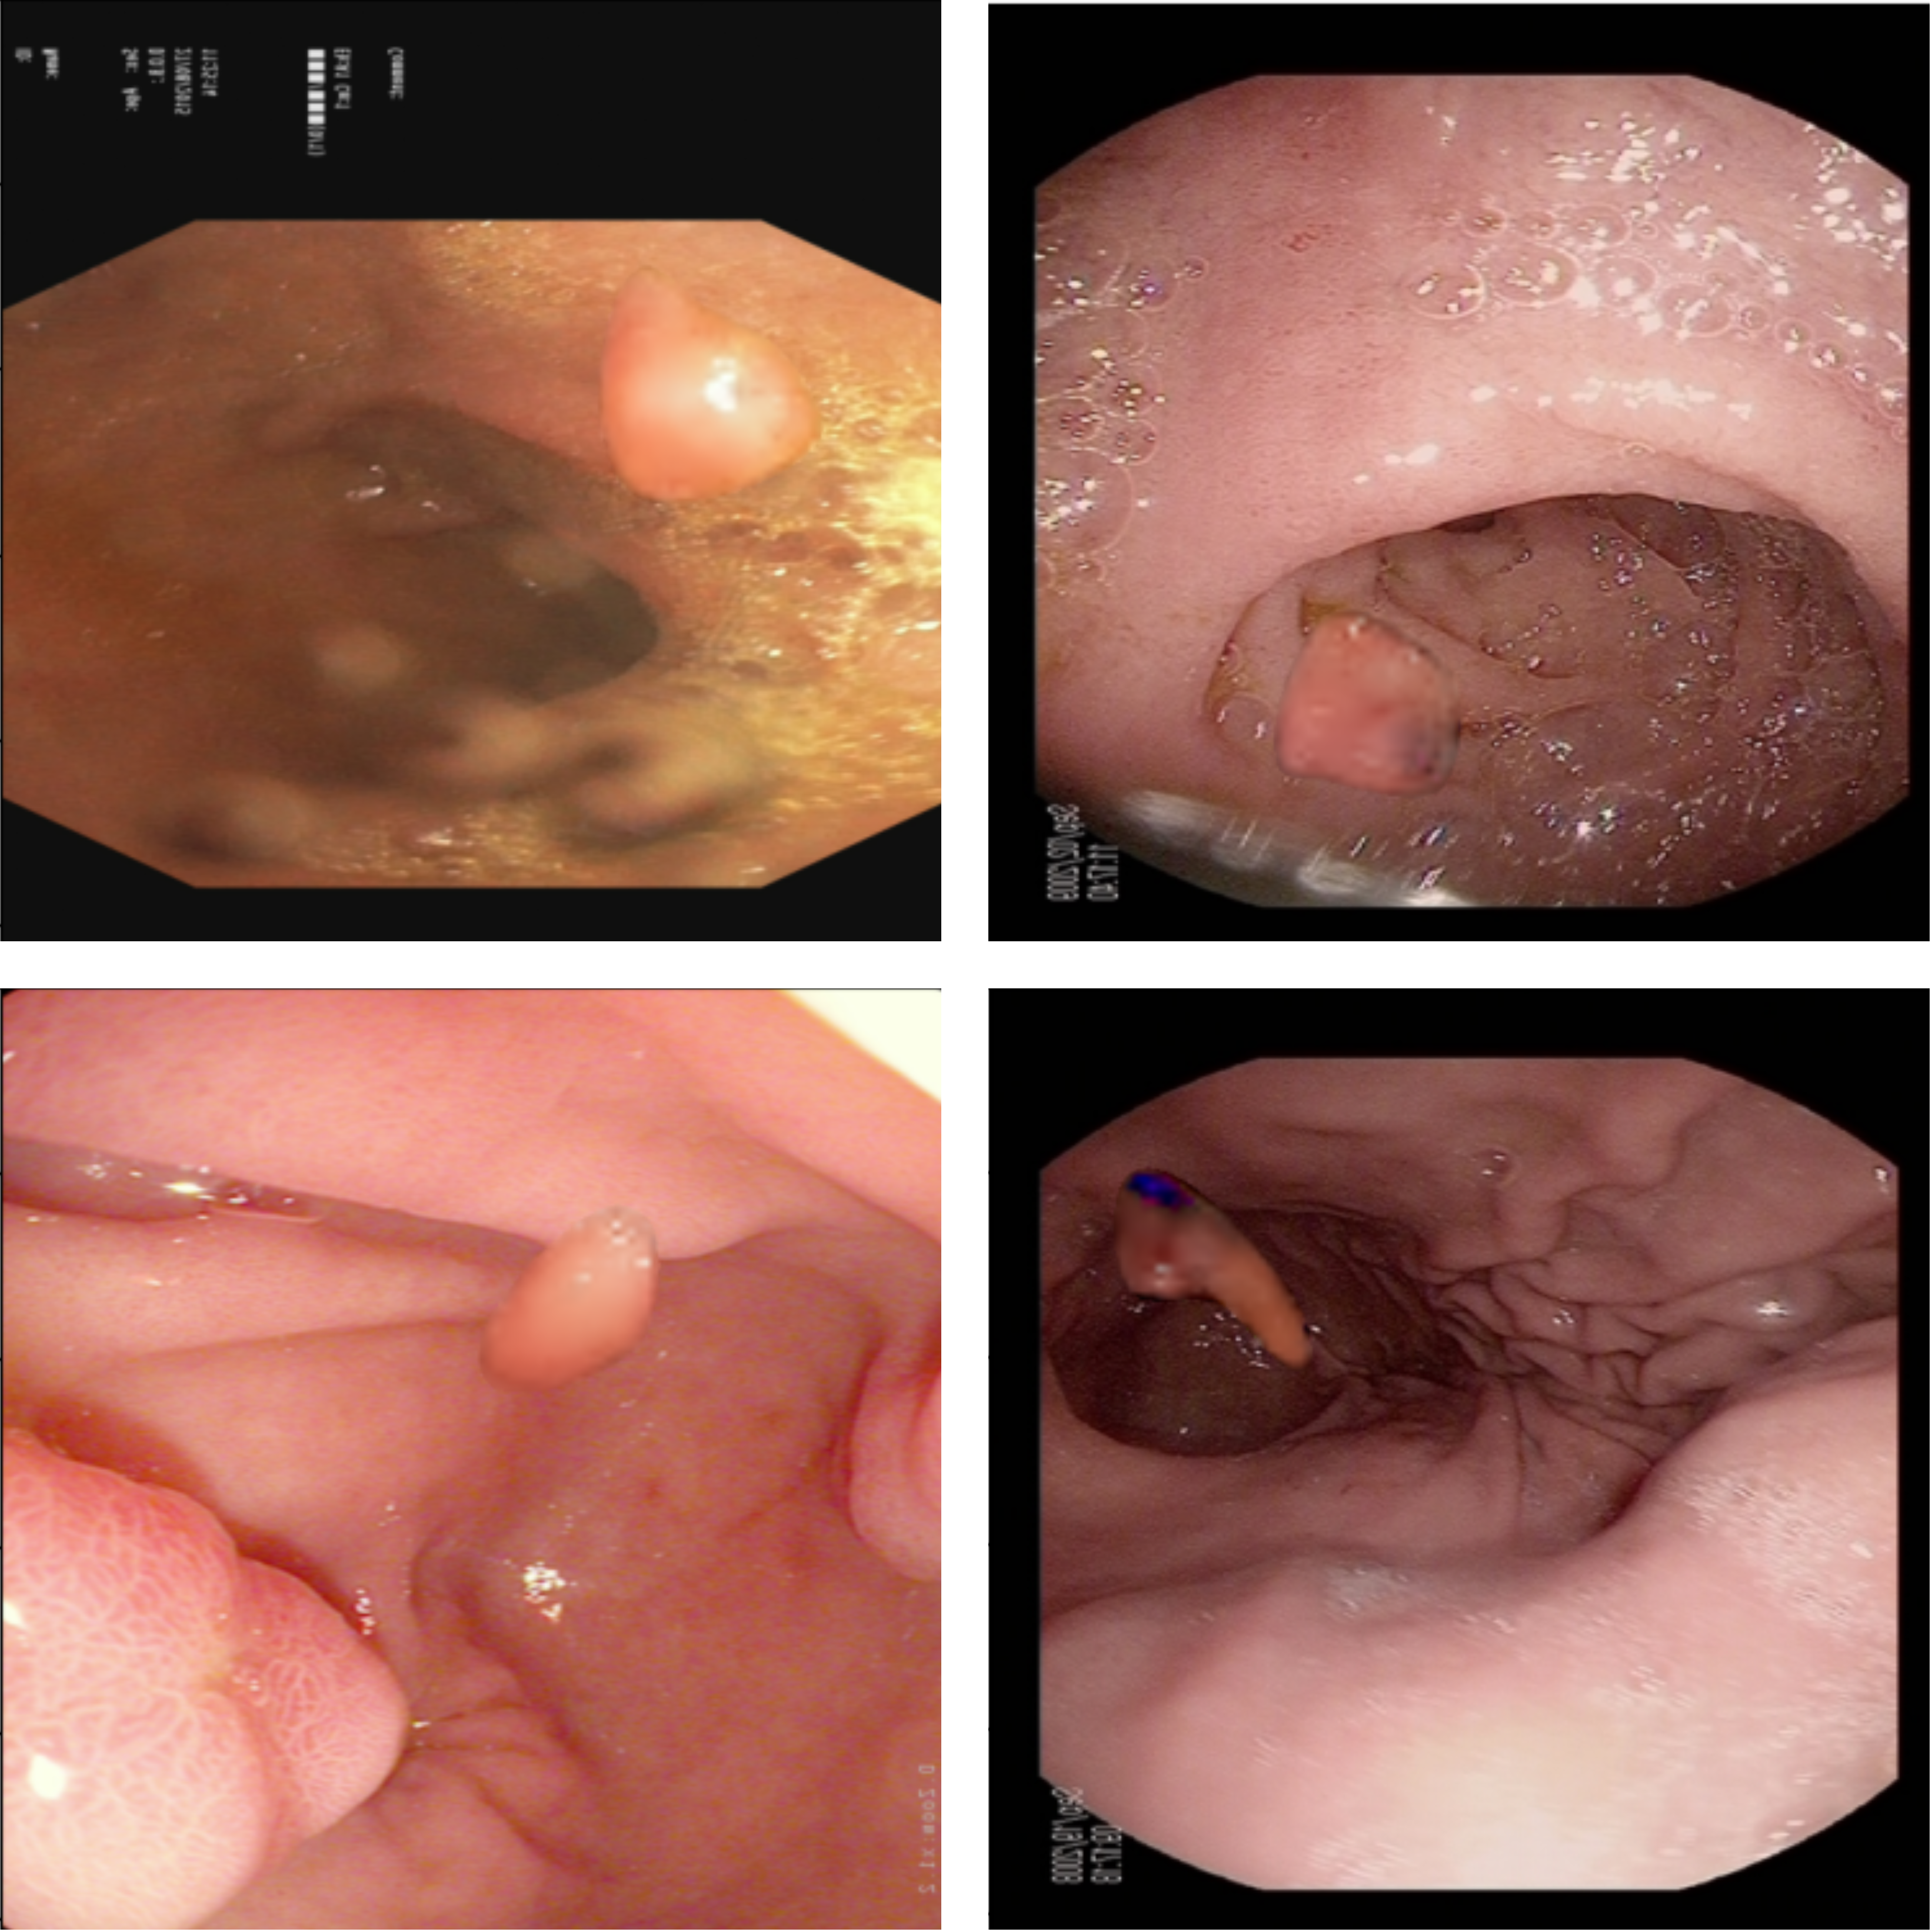
\includegraphics[width=\linewidth]{illustrations/inpainting_examples.png} 
    \caption[GAN-inpainter rexamples]{Example outputs from GAN-inpainter, given unseen inputs taken from an unlabeled dataset. Besides certain colour artifacts, few textural details, and odd lighting, the generated polyps are moderately convincing.}
    \label{fig:inpaint}
\end{figure}


Though this implementation is by no means state-of-the-art, it should nevertheless be sufficient for the purpose of augmentation, considering the principal differences between generated and real polyp images are finer textural details and colour balancing, which are affected by the other augmentations anyway. 

\subsubsection{Geometric and pixel-wise transformations}
The data was augmented using the \textit{albumentations}~\cite{albumentations} library for python, which defines a large number of transformations for use in deep learning. To establish which of these augmentations are suitable, one first needs to establish which invariances the model(s) in question should exhibit.~\Cref{tab:vanilla_aug} below provides descriptions of the invariances required in the model, and the albumentation function that corresponds to the required transform. 
\begin{table}[htb]
    \centering
\begin{tabularx}{\textwidth}{|X|X|}
    \toprule
    \textbf{Invariance} & \textbf{Albumentation Function}\\
    \midrule
    Perspective &Flip() \newline RandomRotate90()\\
    Resolution and Zoom & RandomCrop() \\
    Image quality &GaussNoise() \newline ImageCompression()\\
    Camera models&OpticalDistortion() \\
    Lighting conditions & ColorJitter() \\
    \bottomrule
\end{tabularx}
    \caption{Overview of albumentation augmentations}
    \label{tab:vanilla_aug}
\end{table}

The parameters for the respective functions where selected as follows: one transformation was considered at a time, then parameter value(s) that still kept the polyp fairly visible but still sufficiently altered were identified. The augmentations then sample between a range given by this maximum to determine the severity for each transformation. The probability of each transformation was set to 1, such that all transformations given in~\Cref{tab:vanilla_aug} were always applied, albeit with severity being randomly selected from between 0 and the maximum as previously determined. Thus, though all the transformations were always applied, some may not have any effect if the sampled severity was close to zero. Augmentation examples without the inpainter are shown in~\Cref{fig:sample_augmentations}.

\begin{figure}
    \centering
    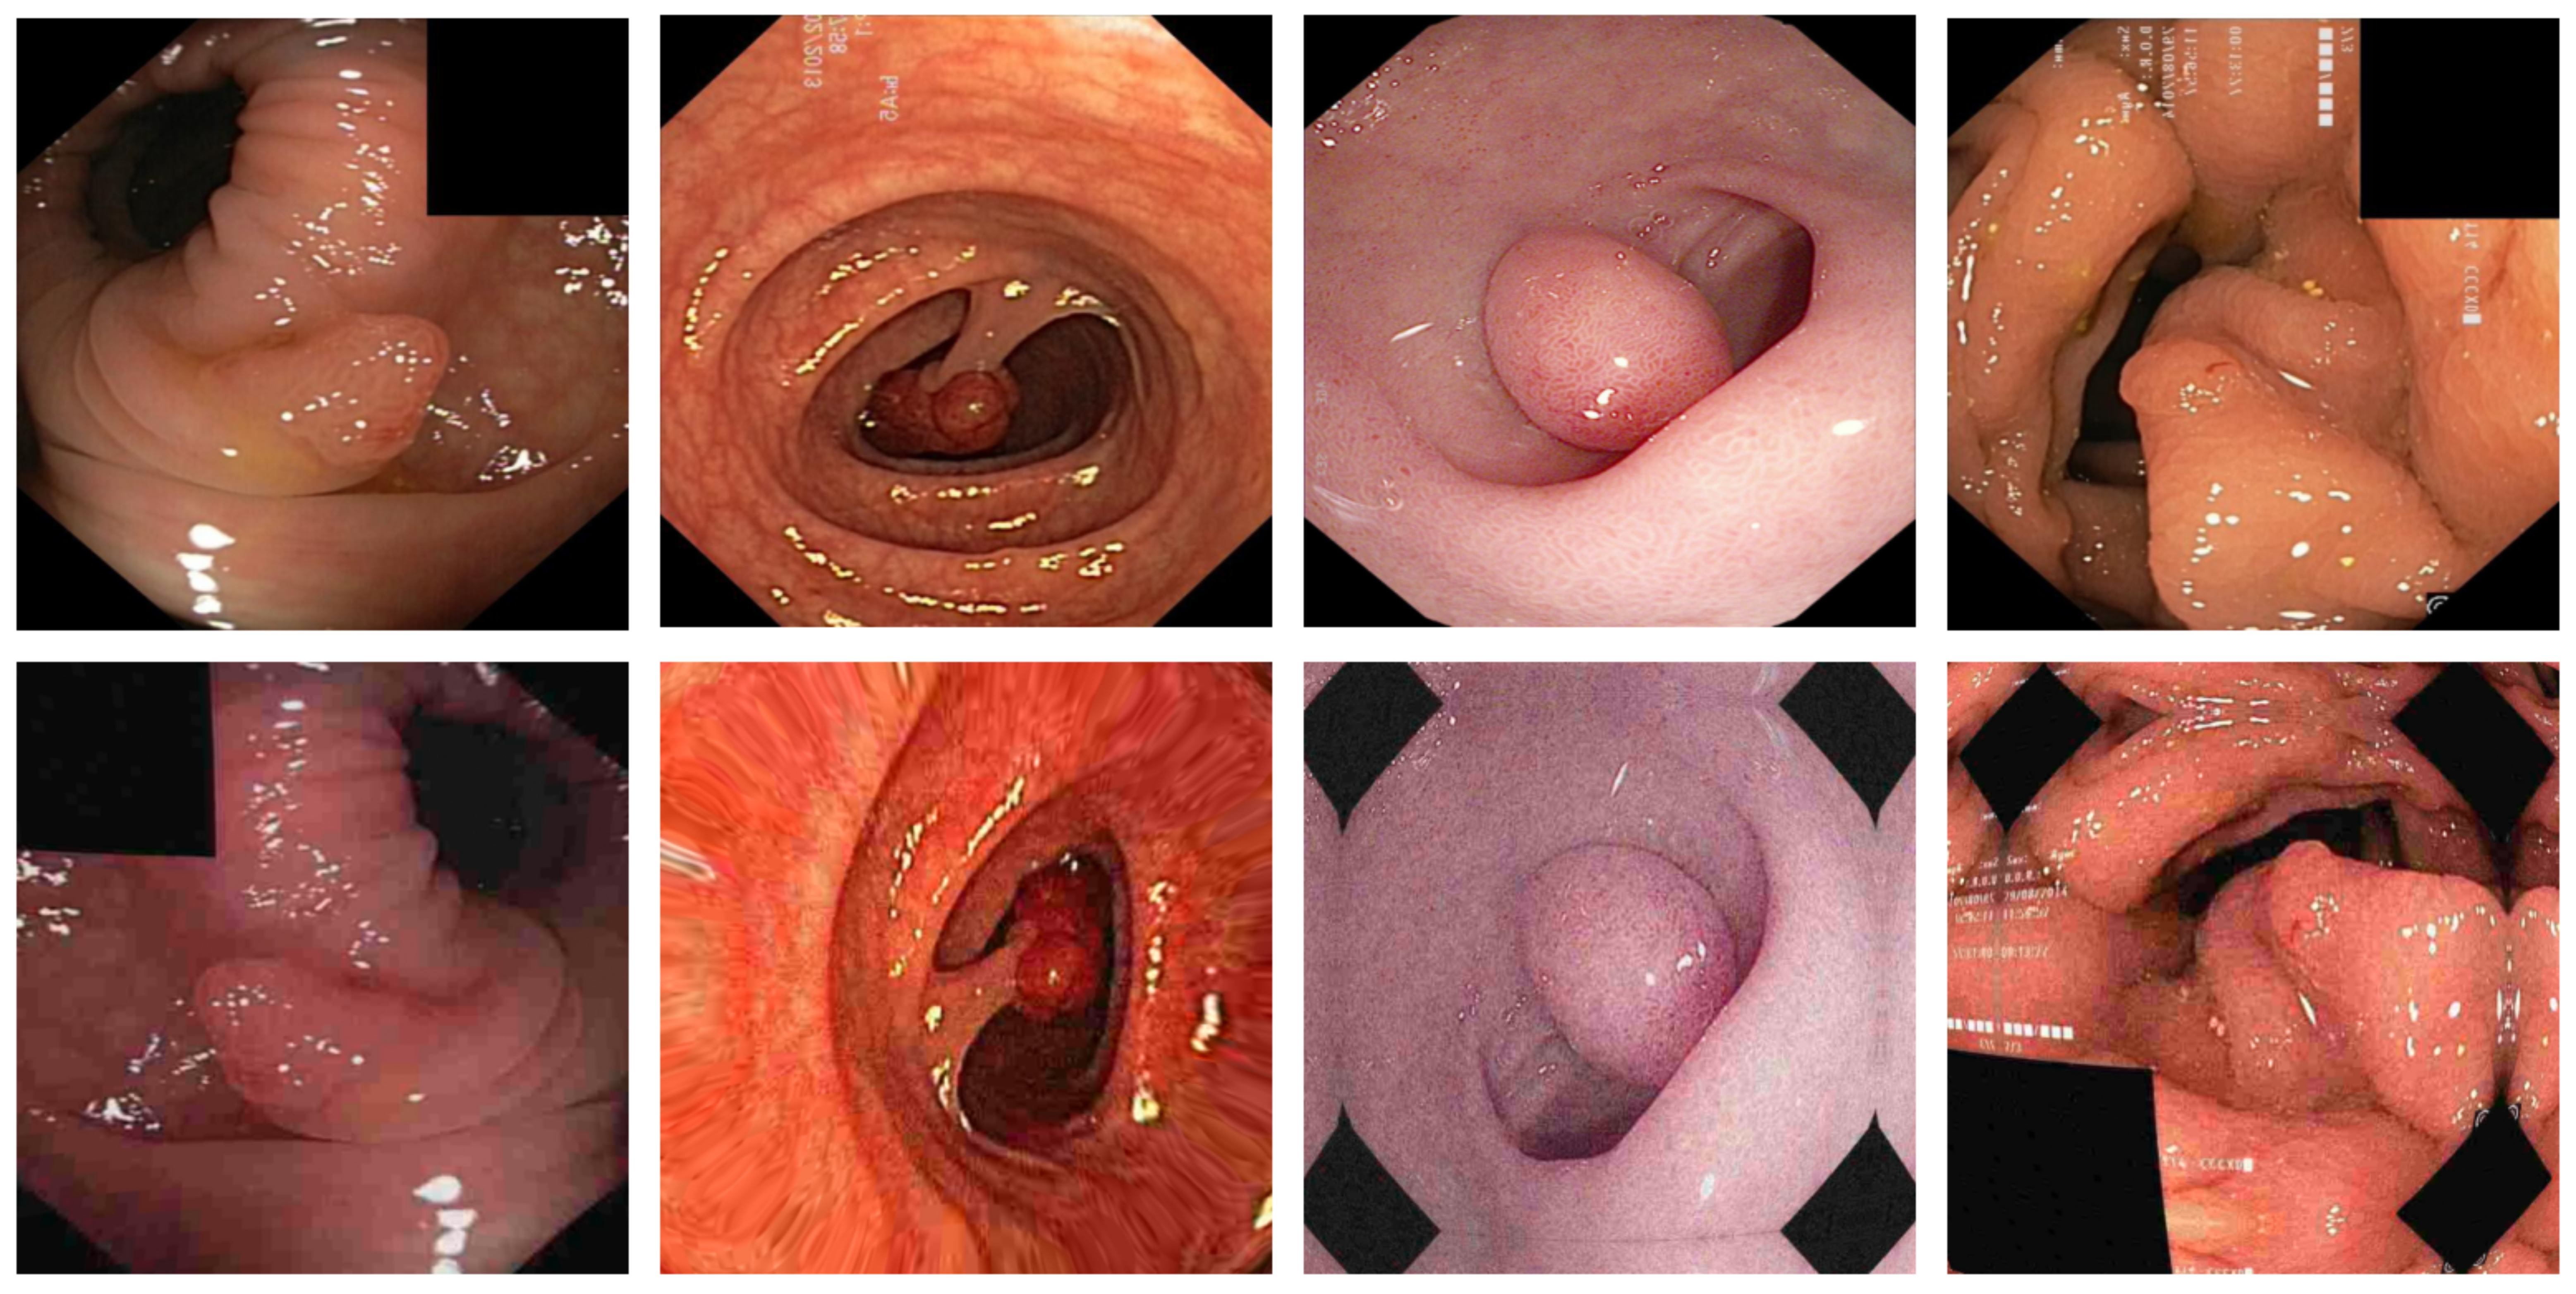
\includegraphics[width=\linewidth]{illustrations/augmentaion_examples.png}
    \caption{Sample Augmentations without inpainter.}
    \label{fig:sample_augmentations}
\end{figure}

It should also be noted that this set of augmentations, even including the inpainter, is of course not complete, in the sense that it accounts for all variability that one might expect in practice. As discussed previously it nevertheless may suffice to model a limited space of these transformations, as it increases the likelihood of learning generalizable features. 

Moreover, the above augmentations are not necessarily optimal, and the selected parameters are not likely to result in the best possible generalizability. In an engineering setting, the choice of augmentations should be tuned and prototyped, but for the purpose of this thesis the simple approach as outlined above is sufficient. 


\subsection{Quantifying Segmentation Consistency}

In~\Cref{consistency_conceptual}, consistency was defined as the property of exhibiting invariance to perturbations. In the context of segmentation, this corresponds to the ability of the model to output the same segmentation mask when the input data is subjected to some perturbation such as those defined in~\Cref{perturbations}.

One simple approach to express this numerically would be to count the number of pixels that do not change in the predicted segmentations when the input is perturbed, and then normalize this with respect to the total number of pixels predicted in both the perturbed and unperturbed images. This, in effect, is equivalent to calculating the \gls{iou} across the perturbed and unperturbed segmentations. However, the ground truth may of course change as a result of the perturbation - if the image is rotated, for example, the segmentation mask should be rotated accordingly. If an image is globally distorted in some way, the segmentation should exhibit the corresponding distortion. This, of course, all needs to be taken into account. This can be achieved by discounting the pixels in the predictions that are expected to change from the overall count. This quantity can be expressed as follows:

Let \(Y:=\{y,\hat{y}:=f(x)\}\) be the set consisting of the segmentation labels (masks) and predictions for the unperturbed samples, where \(f(\cdot)\) as before denotes the model. Let \(\epsilon(\cdot)\) be some perturbation function. Then, let \(A:=\{a:=\epsilon(y),\hat{a}:=f(\epsilon(x))\}\) be the set consisting of segmentation predictions and masks when the input is subjected to a perturbation. Segmentation consistency can then be quantified as:

\begin{equation}
    \mathcal{C}(A,Y) = \frac{\sum\{y \cap a \cap \hat{y} \cap \hat{a} \}}
    {\sum\{ y \cup a \cup \hat{y} \cup \hat{a} \}}
\end{equation}

A visualisation of this metric at work is shown in~\Cref{fig:consistency_example}.

\begin{figure}[htb]
    \centering
    \includegraphics[width=\linewidth]{illustrations/consistency_examples.png}
    \caption[Segmentation Consistency Visualization 1]{Examples of consistency and inconsistency calculation when subjected to a non-label-altering perturbation, in this case additive noise. The consistency for this sample (when thresholded) is 0.68 and inconsistency 0.32, meaning that 64\% of the pixels constitute consistent predictions across the two inputs.}
    \label{fig:consistency_example}
\end{figure}

Using this formulation, higher is of course better. For the purpose of developing a loss function, however, it is useful to instead quantify \textit{inconsistency}. This can be expressed in much the same manner, but using the symmetric difference operator, i.e \(A \ominus B = A \cup B - A \cap B\): 
\begin{equation}\label{eq:inconsistency}
    \overline{\mathcal{C}}(A,Y) = \frac{1}{\sum\{y \cup a \cup \hat{y} \cup \hat{a} \}} \sum \{y\ominus\hat{y}\ominus a\ominus\hat{a}\}
\end{equation}
These formulations are, of course, related by:
\begin{equation*}
    \mathcal{C}(A,Y) = 1-\overline{\mathcal{C}}(A,Y)
\end{equation*}

This notion of inconsistency then corresponds to counting the number of pixels that change after the input is subjected to a perturbation - \(\hat{a}\ominus \hat{y}\), but discounting those we expect to change, \(a\ominus y\). This is also shown in ~\Cref{fig:consistency_example} and~\Cref{loss_fn}.

It is worth noting that consistency is maximized - and thus inconsistency minimized - not only if the predictions are both correct and consistent with one another, but also if the predictions are both incorrect, as long as whatever change that occurs corresponds to the expected change. This is illustrated in~\Cref{loss_fn}.
\begin{figure}[htb]
    \includegraphics[width=\linewidth]{illustrations/loss_visualisation.drawio.png}
    \caption[Segmentation Consistency Visualization 2]{Visualisation of consistency calculation when subjected to a label-altering perturbation, where white is a positive prediction. Note that \(\overline{\mathcal{C}}\) is zero regardless of prediction correctness so long as it changes in the expected manner. Note also that the symmetric difference operators are associative. Left shows an instance of consistent and partially incorrect predictions, and right shows an instance of inconsistent and partially correct predictions.}
    \label{loss_fn}
\end{figure}  
    
Moreover, note that this metric does not presuppose what transformation has occurred. In~\Cref{loss_fn}, for instance, the change induced by the perturbation may correspond to simply moving the polyp in the image (and replacing the empty space with a believable background), or it may correspond to a rotation by 90 degrees. How this should be analyzed with respect to consistency is up to interpretation - one can argue that a rotation should rotate the incorrect predictions as well, or one can argue that it should only rotate the correct component of the prediction. For simplicity, Consistency Training is based on the latter interpretation. This will be discussed in further detail in~\Cref{conclusion}.

\subsection{Inconsistency Loss}
Inconsistency as expressed in~\Cref{eq:inconsistency} is not differentiable, and thus it cannot in its current state be used as a part of a loss function. This, naturally, limits the utility of the idea somewhat. Thus, a smooth extension of this metric is needed which can be achieved in much the same way as how the Jaccard loss can be derived from the Jaccard index - i.e by using differentiable versions of the set functions. 

We can extend the definition of the symmetric difference to \(\Theta(A,B) = A(1-B) + B(1-A)\). This, naturally, is equivalent to the standard symmetric difference if the values of A and B are binary. Similarly, the union operator can be extended as \( \bigcup(A,B) = A+B-AB\), and the intersection operator as \( \bigcap(A,B) = AB\). Like its binary equivalents, these operators maintain their associative and commutative properties. One can optimize for consistency by replacing the operators in~\Cref{eq:inconsistency} with these functions, which in turn can be used as a loss function:

\begin{equation}
    L_c(y, \hat{y},  a, \hat{a}) = \sum \frac{\Theta(y, \hat{y},  a, \hat{a})}{\bigcup(y, \hat{y},  a, \hat{a})}
\end{equation}

This loss function will from this point be referred to as the \gls{sil}. 

\subsection{Adaptive Loss Weighing}
    Naturally, using \gls{sil} as a loss function on its own is not really useful since it only expresses inconsistency, and is to a large extent agnostic to whatever object it is trying to segment. For instance, if the perturbation being performed is simply additive noise, the loss is equally well minimized by predicting that every pixel is positive as it is by segmenting the polyps alone. Consequently, it has to be combined with a some conventional segmentation loss, for instance Jaccard loss. A simple way to do this would be to simply add them together and normalize, i.e:
\begin{equation*}
    L(Y, A) = \frac{1}{2} \big[L_{seg}(Y)+L_c(Y,A)\big]
\end{equation*}
Preliminary experiments showed that this, however, exhibited some degree of instability. The model would readily get stuck in local minima where its predictions were indeed consistent, but also consistently predicting artifacts. Examples of this can be found in~\Cref{non_weighted_ctraining}. 

To mitigate this, it is possible to employ a weighing strategy. Instead of simply adding the respective losses together, one may weight the individual components adaptively according to the \gls{ind} segmentation performance. This way, the model will learn to predict generally correct segmentations early in the training, then start weighing consistency and as a result generalization more and more as the model sees improvements to its segmentation performance:
    \begin{equation}
        L = (1-IoU)\times L_{seg} + IoU \times L_c
    \end{equation}
Using this formulation, the model will start off trying to learn features that contribute to generally improved segmentation performance, then as segmentation performance improves start principally focusing on learning to be consistent. If the model starts veering into areas in the loss-landscape that constitute poor segmentation performance, it will self-correct by weighing the segmentation loss more. In the implementation used in this thesis, these \gls{iou} weights were calculated on a per-batch basis such that the model can quickly adapt if either of the respective objectives exhibit a degradation in performance during training. 

\subsection{Conventional Data Augmentation and Consistency Training}\label{cons_vs_aug}
    At this point, one may easily make the argument that Consistency Training is merely a somewhat more elaborate form of regular data augmentation. To some extent, this argument is well-founded; data augmentations are after all a form of perturbation, and one may argue that \gls{erm} is the mechanism by which consistency across these perturbations is minimized. There are, however, a number of nuances that separate the two methods, as will be discussed below and elaborated upon through mathematical analysis in~\Cref{discussion}. 
    
    With conventional data augmentation, one might assume that the model learns to be invariant to the augmentations as a byproduct of minimizing the empirical risk. By extension, it is assumed that the model will learn features that are equally performant across augmentations. After all, the risk-minimizing configuration is in this case that which exhibits the highest degree of performance when averaged across both augmented and non-augmented images. 
    
    This, however, is not necessarily the case. To illustrate, consider a pipeline intended to segment melanomas. As mentioned in~\Cref{gen_failure_med}, the models in such pipelines are often sensitive to skin-tone. Let us assume that the dataset consists primarily of patients with light complexions, and that data augmentation is used in an attempt to combat any bias as a result of this unbalanced dataset. For simplicity, let us assume that the only augmentation used is transforming the image with colour-jitter with probability \(p=0.5\). In theory, the empirical risk will be best minimized by learning features that do not consider colour and thus skin-tone at all, and instead simply learn to consider the shapes and sizes of the melanomas, the irregularity of which is typically considered a the principal hall-mark of melanomas. 
    
    This is unlikely for two reasons: first, it presupposes that the model readily learns these generalizable features in favor of the more predictive but spurious features during gradient decent. Second, it assumes that learning to perform well is equally easy on both the augmented and the un-augmented images. If, for instance, the model can quickly achieve high average performance and thus minimize risk locally by using color features to achieve excellent performance on the non-augmented images, while exhibiting mediocre or even poor performance on the augmented data, it is unlikely that the model will ever exit this extremely broad local minimum in favor of a more shape-biased and generalizable configuration. Moreover, it may be the case that these shape-based features require significantly more parameters in order to be able to model sufficiently and thus that the performance on the augmented data is limited to a much lower upper bound. In this case, the risk will be minimized not by learning features invariant to the transform, but by learning features that result in a sufficient equilibrium of performance across the augmented and unaugmented sets. I.e, it will try to learn predictive but brittle features as much as possible to maximize performance on unaugmented data, but under the condition that the performance does not degrade too much on the augmented data. Consistency training mitigates this by quantifying the inconsistency of the predictor subject to perturbations, and directly minimizing this quantity. Moreover, due to the weighing method used, consistency is also prioritized starting fairly early in gradient descent. 
    
    Thus, though the two methods share similar traits, they are distinct. Consistency Training can however as mentioned in~\Cref{introduction} be considered an alternative to conventional data augmentation; in pipelines wherein data augmentation is used, one can implement Consistency Training instead so long as there is a suitable method by which to quantify inconsistency. 

\subsection{Putting it all together}
To summarize, Consistency Training is based on the idea that a model necessarily must have learned generalizable features if it has learned invariance to all possible perturbations that do not affect the causal structure of the problem. This is achieved using a perturbation model \(\epsilon(\cdot)\), and a loss function which quantifies the inconsistency of the model when subjected to this perturbation. This loss term then has to be incorporated into the final loss function along with a task-specific loss, hence the adaptive loss weighing. The overall algorithm training process is shown in~\Cref{alg:consistency}:
\begin{algorithm}[htb]
    \caption{Consistency Training}\label{alg:consistency}
    \begin{algorithmic}
    \For{$epochs$}
        \For{$\left(batched\right) {x,y} \in dataset$}
        \State $x_a, a = \epsilon(x, y)$
        \State $\hat{y} \gets f(x)$
        \State $\hat{a} \gets f(x_a)$
        \State $\Bar{\mathcal{C}} \gets \frac{\Theta(\hat{x}, \hat{a},x,a)}{\bigcup(\hat{x}, \hat{a},x,a)}$
        \State $k \gets IoU(x,y)$
        \State $\mathcal{L} = (1-k) \mathcal{J}(x,y) + k \Bar{\mathcal{C}}$
        \State $f(\cdot) \gets optimizer\_update(\mathcal{L})$
        \EndFor
    \EndFor
    \end{algorithmic}
\end{algorithm}


\section{Consistency-trained Ensemble Models}
As mentioned in~\Cref{background}, ensemble-based models have demonstrated high degrees of generalizability~\cite{divergentnets, endoensemble}. Assembling predictors trained with Consistency Training into an ensemble is as a result a simple but effective means by which generalizability can be further increased. 

This can be achieved fairly simply by leveraging multiple identically trained models, such as the dual-decoder DeepLabV3+ - or indeed any model, as will be demonstrated in~\Cref{experiments}. These models can then be used to generate a unique segmentation probability map for each model. This can then be combined into a heatmap, which can then in turn be used to facilitate prediction through the use of any number of consensus methods. In this thesis, the ensembles were implemented to predict according to a simple majority-vote, i.e by thresholding the probability heatmap such that all pixels with probabilities above 0.5 were considered as positive predictions. This is illustrated in~\Cref{fig:ensemble_setup}.

\begin{figure}[htb]
    \centering
    \includegraphics[trim=1.5cm 16cm 0cm 4cm, clip, width=\linewidth]{illustrations/ensemble_config.pdf}
    \caption{Implementation of Ensembles}
    \label{fig:ensemble_setup}
\end{figure}

As mentioned in~\Cref{background}, ensemble models can be considered a form of Bayesian marginalization. As a result, the model is less likely to be affected by underspecification by virtue of the fact that whatever variability in the space of features that a predictor can learn is to some extent accounted for.  

\section{Summary}
This chapter has covered the implementation and theoretical basis for the methods introduced in this thesis. The \textbf{dual decoder DeepLabV3+} aims to increase generalization by constraining the models' latent feature space through the use of image reconstruction as an auxiliary task. \textbf{Consistency training} aims to increase generalization by explicitly optimizing for consistent predictions across perturbed and un-perturbed inputs. These perturbations are application-dependent, and are in this thesis implemented as a carefully designed set of augmentations, consisting of conventional image transformations and a generative inpainting model. Finally, an \textbf{ensemble model} is implemented by combining multiple dual-decoder DeepLabV3+ models trained with Consistency Training. 
    \chapter{Experiments and Results}\label{experiments}
%Experiments intro


\section{Datasets}
%Datasets intro here
\autoref{tab:datasets} shows the size, image resolutions and availability of the respective datasets. 

\begin{table}[h]
    \centering
   \begin{tabularx}{\linewidth}{XXXX}
    \toprule
    Dataset & Resolution & Size & Availability \\
    \midrule
    Kvasir-Seg & Variable & 1000 & Public \\
    Etis-LaribDB & 1255x966 & 196  & Public \\
    CVC-ClinicDB & 388x288 & 612  & Public \\
    EndocCV2020 & ? & ?  & Request \\
    \bottomrule
\end{tabularx}
    \caption{Dataset Overview}
    \label{tab:datasets}
\end{table}

EndoCV2021 should also have been included, ideally, for better comparison to the results published in their proceedings, however since this dataset was unavailable at the time of writing this thesis, this was, unfortunately, not possible. 
\section{Metrics}
    %Intro here
    \subsection{IoU}
    The most natural way to quantify generalizability is, of course, simply evaluating the predictors on in-distribution and out-of-distribution data, then considering the difference. There are, naturally, several performance measures that can be used to this end, the most natural being IoU or the dice coefficient. The predictors were as such evaluated using the IoU across each of the selected datasets. 
    
    \subsection{Detection AUC}
    However, since the provided segmentation masks are not necessarily completely accurate to the pixel-level, and since a polyp-segmentation system would in principle be used primarily as an explainable detection method, a  more pertinent metric is instead simply considering the proportion of polyps that the predictor has managed to segment to any extent at all as a correct prediction. I.e, it may be sufficient that the predictors segment half of the polyp, since this will at least bring the relevant area to the attention of whatever technician is conducting the endoscopy. Increasing detection rates is, after all, the primary concern, and so long as all polyps in a given image are detected, it matters little that some proportion of the pixels corresponding to these polyps are misclassified.
    
    To quantify this, it is possible to simply consider any segmentation above a given IoU threshold as correct, and thereafter compute the precision and recall. 
    
%    Connected component discussion here? I.e metrics that handle multiple polyps in one image
    
    There is of course not one specific threshold that would alert the endoscopy technician to the presence of polyps. Thus, it is better to instead consider the area under the receiver-operator characteristic curve.
    
    
    \subsection{SIS and SIS-AUC}
    As discussed in previous chapters, it is not necessarily the case that \gls{ood} datasets are available, hence the need for a validation procedure that can operate on \gls{ind} data but nevertheless presents some indication of the generalizability of the predictor. To this end, \gls{sis} was introduced. To establish to which extent \gls{sis} really can serve as a surrogate for \gls{ood} dataset evaluation, the area under the \gls{sis} curve across severity levels was also used as an evaluation metric.  
    
    \section{Ablation Study}
    % To investigate the impact of each of the respective components of the new pipeline, and the possible dynamics between them, an ablation study was conducted. Every combination of validation procedure, loss function, model architecture and augmentation strategy were tested. 
    \subsection{Model Baselines and Training}
        In order to evaluate the generalizability of the aforementioned methods sufficiently, they need to be tested across a range of different models, namely DeepLabV3+, \gls{fpn}, UNet, Tri-Unet, and InductiveNet . As such, baseline generalizability metrics were collected for these models, wherein they were trained without augmentation, using \gls{ind}-evaluation, and vanilla Jaccard loss. The hyperparameters were determined experimentally, and can be seen in Table \ref{table:hyperparameters}. Unless otherwise specified, default values were used. 
        \begin{figure}[h]
            \centering
        \begin{tabularx}{\linewidth}{XXX}
        \toprule
        \multicolumn{3}{c}{\textbf{Pipeline Configuration}}\\
        \toprule
        Component & Type & Hyperparameters \\
        \midrule
        Dataloader & - & \(batch\_size = 8\) \\
        && \(\hbox{train/val/test split} = 80/10/10\)\\
        \midrule
        Optimizer & Adam & \(lr = 0.00001\)\\
        \midrule
        Scheduler & Cosine Annealing w/ Warm Restarts & \(T_0=50\) \\
        & & \(T_{mult}=2\) \\
        \midrule
        Evaluation & Loss-based Early Stopping & \(epochs=250\)\\
        \bottomrule
        \end{tabularx}
            \caption{Hyperparameters for baselines}
            \label{table:hyperparameters}
        \end{figure}
        Ten predictors were trained for each model in order to ascertain statistical significance, and evaluated according to the aforementioned metrics. 
        
    
    \input{tables/ablation_auc}

        
     \subsection{Ensembles}
        \subsubsection{Singular Ensembles}
        \subsection{Diverse Ensembles}
        \subsection{Trained Multistage Ensembles}
        
    \chapter{Discussion}\label{discussion}
\section{}
\section{Auxilliary findings}
    \chapter{Conclusion}\label{conclusion}

% \section{Summary}
% The goal of this work has been to develop novel methods of increasing the generalizability of deep learning models, as well as to further the understanding of the relative impacts of more conventional components of the deep learning pipeline.

% Several methods were proposed to this end, namely DD-DeepLabV3+, Consistency Training, generative polyp inpainting, and the use of ensembles. Among these methods, Consistency Training had the most significant impact and appears to be the most promising with regards to further development. 

% There are a multitude of improvements that could be made for every tested method, and there is much to be gained from more in-depth analysis and experimentation with regards to the relative impacts of all tested methods. 

% Though generalizability remains an open and multifaceted problem, there are evidently multiple promising directions of further study which may yet prove to alleviate generalization failure or at the very least facilitate a deeper understanding of generalizability. In particular, Consistency Training, and in general notion of perturbation consistency, exhibits significant potential towards mitigating generalization failure.
 
\section{Summary}
The goal of this work has been to develop novel methods of increasing the generalizability of deep learning models, as well as to survey the relative impacts of more conventional components of the deep learning pipeline. This was achieved as follows:

\Cref{background} provided an overview of deep learning, segmentation, and delved further into why such systems so readily fail to generalize, starting from first principles and analyzing the shortcomings of \gls{erm}. This was then connected to recent analyses of generalizability failure, including the notion of underspecification and shortcut learning. Finally, known methods of increasing generalization as presented in EndoCV2021 and elsewhere in the literature were then discussed and analyzed with respect to the established theory. 

This was then in turn used to inform the development of the methods discussed in \Cref{methods}, including a novel training paradigm, augmentation technique, model architecture and ensemble models. Each of these methods were also discussed with respect to the theory explored in \Cref{background}.

Several experiments were then conducted in \Cref{experiments} in order to ascertain the impact of the proposed methods:
First, baseline generalizability metric were collected for five separate models. The findings supported the notion that larger models are more prone to generalizability failure, as demonstrated by the significant gap between the Unet and the TriUnet. The use of a secondary decoder in the DD-DeepLabV3+ model was shown to have negligible impact, despite reducing performance variability. It was hypothesized that this is due to the encoder already learning domain- and dataset-independent features. 

In the next experiment, data augmentation was shown to increase generalizability by a considerable margin. Synthetic augmentation via inpainting was shown to hamper this improvement when used in conjunction with regular augmentation, but this finding was deemed inconclusive due to the relatively low performance of the inpainter. 
The impact of consistency training was then tested and compared to regular data augmentation and no augmentation. The results show that consistency training outperforms regular data augmentation by a considerable margin on the most difficult of the three \gls{ood} datasets. 

Finally, predictors trained according to the best methods as identified in the previous experiments were then combined into ensembles. The results demonstrated the generalizability of ensemble-based methods, but further analysis did not sufficiently corroborate that this improvement can be attributed to ensembles mitigating underspecification. 

The results from this experiment was then discussed in \Cref{discussion}. Limitations of the experiments were noted, along with their practical impacts and possible directions of further study and potential ways to improve the methods proposed in this thesis. 


\section{Contributions}
The main contributions in this thesis can be regarded as twofold:

First, the thesis introduces a new way of thinking about generalization as consistency to perturbations. This informed the development of Consistency Training, which was shown to increase generalizability by a greater margin than all other tested methods, including data augmentation. This framework, and the potential improvements that can be made upon it as suggested in \Cref{discussion}, shows good promise with regards to further increasing generalizability. 

Second, this work provides an exploratory overview of how generalizability is affected by the choice of model architecture, augmentation strategy, and the use of ensembles. Though most of the findings corroborated the literature, there were a fair number of surprising results that warrant further investigation, in particular with regards to the impacts of the tested methods relative to one another. For one, the effect of multitask learning and generally the the choice of model architecture was practically negligible. With the exception of TriUnet, every tested model exhibited practically identical performance. Ensembles, though exhibiting statistically significant impact, resulted in somewhat marginal improvements on generalization, especially in comparison to the use of data augmentation and consistency training. As discussed in \Cref{discussion}, this raises doubts as to the veracity of findings in other literature, where data augmentation is rarely accounted for when performing comparisons. Hopefully, the findings in this thesis demonstrates the need for a more structured approach to the design of experimental methodologies intended to analyze generalization, wherein the constituent components of the pipeline are sufficiently controlled. 

\section{Future Work}
There are a myriad of promising directions for further work. These are detailed in \Cref{discussion} and can be summarized as follows:

There are several ways to improve Consistency Training. One may for instance modify the segmentation inconsistency loss as outlined in \Cref{new_closs}. It is also possible to incorporate the notion of consistency in more advanced pipelines, such as through denoising networks as outlined in \Cref{denoising}. Adversarial sampling of perturbations or otherwise modifying the perturbation model may also have merit.  

Further investigating the effect of multiple-decoder models may also prove insightful, in particular as a countermeasure to underspecification. Analyzing the latent representations and the differences that these decoders induce may also provide a better understanding of what the encoders actually learn, and corroborate the hypothesis made in \Cref{models} that they learn dataset- and thus task-invariant features. 

Repeating the experiments performed in this thesis without pretraining may also be interesting. There may for instance be a relationship between pretraining and the aforementioned tendency of encoders to learn task-independent features which such experiments would highlight.  

As this thesis merely explored the impacts of model architectures, data augmentation and ensemble models on a surface level, there is naturally space for more in-depth exploration of the relationships suggested by the findings in \Cref{experiments}. In particular, a more in-depth analysis of the impact of data augmentation is warranted, in particular in regards to the relative impacts thereof in comparison to other methods. A meta-analysis of the findings in EndoCV2021 wherein the same augmentation method is kept across all submitted methods may for instance be a useful point of further study towards developing more robust experimental methods to evaluate generalization. 
    \backmatter{}
    \printbibliography
    \chapter*{Appendix A: Code Access} \label{code_data}
\addcontentsline{toc}{chapter}{Appendix A}
All relevant code and data can be found on the GitHub repository: https://github.com/BirkTorpmannHagen/Master

\chapter*{Appendix B: p-values}\label{p-values}
\addcontentsline{toc}{chapter}{Appendix B: p-values}

\begin{figure}[hbt]
    \centering
    \includegraphics[width=\linewidth]{illustrations/model_pvals.eps}
    \caption{Two-sided independent t-test p-values between models for all datasets}
    \label{models_pvalues}
\end{figure}
% inpainter
\begin{table}[htb]
    \centering
    \begin{tabularx}{\linewidth}{lXXXX}
    \toprule
     Model & CVC-ClinicDB & EndoCV2020 & Etis-LaribDB & Kvasir-SEG\\
    \midrule
    DD-DeepLabV3+ & 0.04454 & 0.95857 & 0.12809 & 0.30201\\ 
    DeepLab & \textbf{0.0096} & 0.08898 & 0.11401 & 0.31065\\ 
    FPN & 0.13769 & 0.95284 & 0.17806 & 0.16613\\ 
    TriUnet & 0.13412 & 0.31111 & 0.19913 & 0.91489\\ 
    Unet & 0.01069 & 0.15406 & 0.02715 & 0.36489\\ 
      \bottomrule
    \end{tabularx}
    \caption[T-test results inpainting]{p-values for each model and dataset between the IoUs of the given models trained with  versus when trained with conventional data augmentation versus models trained with the inpainter as a component of the data augmentation strategy}
    \label{tab:ttest_per_dataset_inpainter}
\end{table}
\begin{table}[htb]
    \centering
    \begin{tabularx}{\linewidth}{lXr}
        \toprule
        Dataset & U-Statistic & p-Value \\
        \midrule
            Kvasir-SEG & 763.0, p=0.15972 \\ 
            Etis-LaribDB & 545.0, p=0.00163 \\ 
            EndoCV2020 & 851.0, p=0.4169 \\ 
            CVC-ClinicDB & 520.0, p=0.00077 \\ 
        \bottomrule
    \end{tabularx}
    \caption[Mann-Whitney U-test results inpainter averaged across models]{Results from Mann-Whitney U-test for each dataset when comparing the average \glspl{iou} of all models trained with conventional data augmentation versus models trained with the inpainter as a component of the data augmentation strategy}
    \label{tab:ttest_avgs_inpainter}
\end{table}

% consistency training
\begin{table}[htb]
    \centering
    \begin{tabularx}{\linewidth}{lXXXX}
    \toprule
      Model & CVC-ClinicDB & EndoCV2020 & Etis-LaribDB & Kvasir-SEG\\
      \midrule
      DD-DeepLabV3+ & 0.014 & 0.985 & 0.083 & 0.170\\
      DeepLab       & 0.029 & 0.901 & \textbf{0.003} & 0.444\\
      FPN           & \textbf{0.004} & 0.038 & \textbf{0.005} & 0.939\\
      TriUnet       & 0.211 & 0.024 & 0.141 & 0.330\\
      Unet          & \textbf{0.000} & \textbf{0.001} & \textbf{0.006} & 0.899\\
      \bottomrule
    \end{tabularx}
    \caption[T-test results consistency training]{p-values for each model and dataset between the IoUs of the given models trained with consistency training versus when trained with data augmentaion}
    \label{tab:ttest_per_dataset_consistency}
\end{table}
\begin{table}[htb]
    \centering
    \begin{tabularx}{\linewidth}{lXr}
            \toprule
            Dataset & U-Statistic & p-Value \\
            \midrule
            Kvasir-SEG & 1066.0 & 0.10293 \\
            Etis-LaribDB & 624.0 & 0.00001\\
            CVC-ClinicDB & 751.0& p=0.00029 \\
            EndoCV2020 & 774.0 & 0.00052    \\
            \bottomrule
        \end{tabularx}
        \caption[Mann-Whitney U-test results consistency training averaged across models]{Results from a Mann-Whitney U-test for each dataset when comparing the average \glspl{iou} across models for Consistency Training vs conventional data augmentation}
        \label{tab:ttest_avgs_consistency}
    \end{table}
    
% Ensembles
\begin{table}[htb]
    \centering
    \begin{tabularx}{\linewidth}{lXr}
        \toprule
        Dataset & U-Statistic & p-Value \\
        \midrule
        Kvasir-SEG & 1150.0 & 0.00074 \\ 
        Etis-LaribDB & 742.0 & 0.0 \\ 
        EndoCV2020 & 1265.0 & 0.00523 \\ 
        CVC-ClinicDB & 1319.0 & 0.01163 \\ 
        \bottomrule
    \end{tabularx}
    \caption[Mann-Whitney U-test results ensembles]{Results from Mann-Whitney U-test for each dataset when comparing the average \glspl{iou} across ensembles consisting of predictors trained with Consistency Training versus predictors trained with conventional data augmentation. Precision limited to 5 significant figures}
    \label{tab:ttest_avgs_ensemble}
\end{table}
    

\newpage
\chapter*{Appendix C: Non-weighted Consistency Training}\label{non_weighted_ctraining}
\addcontentsline{toc}{chapter}{Appendix C: Non-weighted Consistency Training}

\begin{figure}[htb]
    \centering
    \includegraphics[width=\linewidth]{illustrations/artefacts.png}
    \caption[Unweighted Consistency example]{When the consistency term is not modulated dynamically, the model can quickly learn to predict artifacts around the edges of the image. As polyps can rarely be found in these regions, the consistency term is minimized by predicting consistently wrong predictions where there typically are not polyps. }
    \label{fig:non_weighted_ctraining}
\end{figure}

\chapter*{Appendix D: Paper submitted to NeurIPS2022} \label{Paper}
\addcontentsline{toc}{chapter}{Appendix D: Paper submitted to NeurIPS2022}
\setcounter{chapter}{8}
\setcounter{section}{0}
\section*{Paper submitted to NeurIPS2022}
\setcounter{chapter}{0}
\setcounter{section}{0} 
\includepdf[pages=-]{2022_NIPS_paper_Birk.pdf} 



\end{document}
